\documentclass[fleqn,10pt]{article}
\usepackage[utf8]{inputenc}
\usepackage[T1]{fontenc}

% =========================
% Nature Portfolio / Scientific Reports Style
% =========================
\usepackage{graphicx}
\usepackage{amsmath, amssymb}
\usepackage{geometry}
\usepackage{setspace}
\usepackage{booktabs}
\usepackage{longtable}
\usepackage{hyperref}
\usepackage[superscript,biblabel]{cite} % Numbered superscript citations
\usepackage{float}
\usepackage{caption}
\usepackage{subcaption}
\usepackage{multirow}
\usepackage{enumitem}
\usepackage{xcolor}
\usepackage{tabularx}
\usepackage{authblk} % For author affiliations

\graphicspath{{.}{./figures/}}

\geometry{margin=1in}
\onehalfspacing

% =========================
% Title & Author
% =========================
\title{
Decadal Surface Water Dynamics in Bangladesh Using Sentinel-1 SAR:\\
Seasonal Variability, Change Detection, and Trend Analysis (2015--2025)
}

\author[1]{[Author 1 Name]}
\author[2]{[Author 2 Name]}
\affil[1]{[Author 1 Affiliation Details]}
\affil[2]{[Author 2 Affiliation Details]}
\affil[*]{Corresponding author: [Contact Email]} % Replace with actual email

\date{} % Nature typically does not include the date on the title page

\date{}

\begin{document}
\maketitle

% =========================
% Abstract
% =========================
\begin{abstract}
Surface water dynamics play a critical role in the hydrological, ecological, and socio-economic systems of Bangladesh---the world's largest deltaic nation. Persistent cloud cover during monsoon months severely limits optical remote sensing, creating a need for radar-based monitoring approaches. This study presents an 11-year Sentinel-1 SAR time-series analysis (2015--2025) based on 7,891 radar acquisitions, enabling monthly monitoring of surface water dynamics across Bangladesh within the Google Earth Engine (GEE) platform. Monthly surface water maps were generated using seasonally adaptive VV backscatter thresholds calibrated to Bangladesh's four hydrological seasons. From these monthly products, annual water occurrence frequency maps, seasonal water footprints, and inter-annual change detection maps (gain/loss/stable) were derived at national, divisional, and district scales. Decadal-scale trend analysis was performed using Seasonal Mann-Kendall tests and Sen's slope estimators to rigorously identify long-term shifts in surface water extent. The results were validated using a robust dataset of 4,310 monthly balanced field-verified reference points (2025), achieving an overall accuracy of 92.55\% and a Kappa coefficient of 0.85. Area uncertainty bounds were calculated at $\pm0.78\%$ using 95\% confidence interval error propagation from the confusion matrix. The analysis reveals that the mean open surface water area in Bangladesh ranges from approximately 5,678~km$^2$ ($\pm$45~km$^2$, 3.8\% of land area) in January-February to 23,269~km$^2$ ($\pm$182~km$^2$, 15.7\% of land area) during the peak monsoon in July. Over the 11-year period, 3.4\% of the land area remained permanently inundated, while ephemeral water bodies covered an additional 29.2\%. Change detection indicates substantial spatial redistribution of monsoon inundation, with approximately 21.5\% of the 2025 monsoon water extent occurring in areas newly inundated relative to 2015, despite the absence of a statistically significant long-term trend. These results demonstrate the capability of Sentinel-1 SAR time-series analysis for consistent monitoring of seasonal flood dynamics in large delta systems, supporting improved flood risk assessment and water-resource management.

\vspace{0.5em}
\noindent\textbf{Keywords:} Sentinel-1 SAR; Surface water dynamics; Seasonal variability; Change detection; Trend analysis; Google Earth Engine; Bangladesh
\end{abstract}

% =========================
\section{Introduction}
% =========================

Surface water is a dynamic component of the hydrological cycle, with pronounced temporal and spatial variability in low-lying deltaic regions. Bangladesh, situated at the confluence of the Ganges--Brahmaputra--Meghna (GBM) river system, is the world's largest delta system. Approximately 80\% of the country is flood-prone, and surface water conditions directly influence agriculture, fisheries, navigation, drinking water supply, and ecosystem services for over 170 million inhabitants \cite{brammer2014, akter2016, roy2023, gourdji2015}.

Remote sensing provides the only feasible means for systematic, large-scale surface water monitoring. Optical sensors such as Landsat and Sentinel-2 have been widely used for water mapping \cite{pekel2016, pickens2020}; however, their utility over Bangladesh is severely constrained during the monsoon season (June--September), when cloud cover exceeds 80\% on most acquisition dates \cite{uddin2019, hassan2021}. Synthetic Aperture Radar (SAR), operating in the microwave spectrum, overcomes this limitation by providing all-weather, day-night imaging capability. Sentinel-1 C-band SAR, in particular, has become a primary data source for surface water detection due to its free availability, systematic global coverage, and well-characterized backscatter response over water surfaces \cite{torres2012, twele2016, haghighi2022, sayed2023}.

SAR-based water detection exploits the specular reflection properties of smooth water surfaces, which produce characteristically low radar backscatter compared to surrounding land. Numerous studies have demonstrated the effectiveness of VV-polarized backscatter thresholding for water delineation \cite{twele2016, bioresita2018, martinis2009, hossain2024}. However, the majority of SAR-based studies focus on event-specific flood mapping---detecting inundation from individual flood events---rather than characterizing long-term surface water dynamics, seasonal patterns, and inter-annual trends \cite{devries2020}. Recent advancements, such as the NASA JPL Dynamic Surface Water Extent (DSWx-S1) product \cite{nasa2024} and automated recursive classification frameworks \cite{markert2020, ogrady2021}, highlight the growing importance of operational SAR-based water monitoring. Furthermore, most approaches employ static backscatter thresholds, which may not adequately represent the seasonal variability in SAR response caused by changes in wind conditions, vegetation phenology, and soil moisture across Bangladesh's four distinct hydrological seasons. Tran et al. \cite{tran2024} recently demonstrated the utility of Sentinel-1 time series for monitoring dynamic deltas, further justifying the need for adaptive monitoring frameworks.

This study addresses these gaps by presenting a comprehensive decadal-scale analysis of surface water dynamics across Bangladesh using Sentinel-1 SAR data from 2015 to 2025. The specific objectives are:
\begin{enumerate}[nosep]
  \item Generate monthly surface water maps using seasonally adaptive VV backscatter thresholds calibrated to Bangladesh's hydrological seasons;
  \item Map annual water occurrence frequency to classify permanent, semi-permanent, and ephemeral water bodies;
  \item Detect and quantify inter-annual surface water change (gain, loss, stable) between selected years;
  \item Characterize seasonal water footprints across Bangladesh's four hydrological seasons;
  \item Perform decadal trend analysis of surface water extent at national, divisional, and district scales;
  \item Validate SAR-derived water maps against 4,310 monthly balanced field-verified reference points (2025).
\end{enumerate}

The study contributes: (i) the first decadal Sentinel-1 SAR water dataset for Bangladesh, (ii) a seasonally adaptive threshold framework calibrated to deltaic hydrology, (iii) multi-scale analysis from national to district levels, and (iv) a fully reproducible cloud-based monitoring workflow.


% =========================
\section{Study Area}
% =========================

Bangladesh is located in South Asia between latitudes 20\textdegree34$'$ and 26\textdegree38$'$ N and longitudes 88\textdegree01$'$ and 92\textdegree41$'$ E, covering approximately 147,570~km$^{2}$ (Figure~\ref{fig:study_area}). The country is characterized by predominantly flat topography, dense river networks, and extensive floodplains formed by the Ganges--Brahmaputra--Meghna (GBM) river system---the world's largest delta system. Elevation ranges from sea level in the southern coastal zone to approximately 1,000~m in the Chittagong Hill Tracts.

Bangladesh experiences a tropical monsoon climate with four distinct hydrological seasons:
\begin{itemize}[nosep]
  \item \textbf{Dry Winter (December--February):} Minimal rainfall, reduced river discharge, minimum surface water extent.
  \item \textbf{Pre-Monsoon (March--May):} Rising temperatures, occasional thunderstorms, gradual increase in water extent.
  \item \textbf{Monsoon (June--September):} Heavy rainfall contributing 70--80\% of annual precipitation, peak river discharge, maximum surface water extent.
  \item \textbf{Post-Monsoon (October--November):} Recession of floodwaters, gradual contraction of water bodies.
\end{itemize}

Administratively, the country comprises 8 divisions and 64 districts. This study utilizes this administrative hierarchy for multi-scale spatial analysis of surface water dynamics.

\begin{figure}[H]
    \centering
    
\includegraphics[width=1.0\textwidth]{fig1_study_area.png}
    \caption{Study area map of Bangladesh showing the eight administrative divisions, major river systems (Ganges, Brahmaputra, and Meghna), and the geographical setting of the study.}
    \label{fig:study_area}
\end{figure}


% =========================
\section{Data and Materials}
% =========================

\subsection{Sentinel-1 SAR Data}

Sentinel-1 C-band SAR Ground Range Detected (GRD) imagery acquired in Interferometric Wide (IW) swath mode was used as the primary data source. The VV polarization channel was selected due to its well-documented sensitivity to open water surfaces, where smooth water produces low backscatter through specular reflection \cite{twele2016, bioresita2018}. Table~\ref{tab:s1_specs} summarizes the data specifications.

\begin{table}[H]
\centering
\caption{Sentinel-1 SAR data specifications.}
\label{tab:s1_specs}
\begin{tabular}{ll}
\toprule
\textbf{Parameter} & \textbf{Value} \\
\midrule
Satellite & Sentinel-1A/B \\
Product & GRD (Ground Range Detected) \\
Mode & IW (Interferometric Wide) \\
Polarization & VV \\
Spatial Resolution & 10 m \\
Temporal Coverage & January 2015 -- December 2025 \\
Temporal Resolution & 12 days (6 days with dual satellite) \\
Band & Sigma0 (dB) \\
Processing Level & Pre-processed (GEE) \\
\bottomrule
\end{tabular}
\end{table}

\begin{table}[H]
\centering
\caption{Number of Sentinel-1 scenes used per year for Bangladesh.}
\label{tab:s1_count}
\begin{tabular}{lccccccccccc}
\toprule
\textbf{Year} & 2015 & 2016 & 2017 & 2018 & 2019 & 2020 & 2021 & 2022 & 2023 & 2024 & 2025 \\
\midrule
Scenes & 304 & 480 & 612 & 785 & 812 & 830 & 845 & 790 & 815 & 851 & 767 \\
\bottomrule
\end{tabular}
\end{table}

\subsection{Validation Data}

\subsubsection{Field-Verified Reference Data}
The primary reference dataset for accuracy assessment consists of 4,310 spatial-temporal validation observations collected throughout 2025. These observations are derived from a set of fixed field locations (approximately 400 sites) that were physically monitored across the 12 calendar months to capture both dry-season baseline and monsoon inundation states. To establish a robust ground truth, the status of each location during the specific month was rigorously verified through direct field observation and local field knowledge, confirming the true binary classification (1 = Water, 0 = Non-water).

\subsection{Administrative Boundaries}
FAO GAUL Level-1 (divisions) and Level-2 (districts) boundary datasets, accessed through Google Earth Engine, were used for spatial aggregation and multi-scale reporting.

\subsection{Processing Platform}
All SAR data processing, water detection, and product generation were performed in Google Earth Engine (GEE) \cite{gorelick2017}, enabling cloud-based access to the complete Sentinel-1 archive without local data storage or computational infrastructure requirements.


% =========================
\section{Methodology}
% =========================

\begin{figure}[H]
    \centering
    
\includegraphics[width=0.6\textwidth,height=0.28\textheight,keepaspectratio]{fig2_flowchart.png}
    \caption{Methodological framework for decadal surface water monitoring in Bangladesh using Sentinel-1 SAR and seasonally adaptive thresholding.}
    \label{fig:flowchart}
\end{figure}


\subsection{Overview}
The proposed analytical framework (Figure~\ref{fig:flowchart}) consists of five main components:
\begin{enumerate}[nosep]
  \item SAR-based monthly surface water detection using seasonally adaptive thresholds
  \item Annual water occurrence frequency mapping
  \item Inter-annual change detection (gain/loss/stable classification)
  \item Seasonal water footprint analysis
  \item Decadal trend analysis at multiple administrative scales
\end{enumerate}

% --- 4.2 Monthly Detection ---
\subsection{Monthly Surface Water Detection}
\label{sec:water_detection}

For each calendar month and administrative region, all available Sentinel-1 IW GRD scenes with VV polarization were filtered from the GEE archive. The monthly median VV backscatter composite was computed to reduce speckle noise and minimize the influence of transient features \cite{clement2018, pham-duc2017}:

\begin{equation}
\sigma^{0}_{VV,m} = \text{median}\left(\sigma^{0}_{VV,i}\right), \quad i = 1, 2, \ldots, N_m
\label{eq:median}
\end{equation}

where $\sigma^{0}_{VV,m}$ is the monthly median backscatter in decibels and $N_m$ is the number of Sentinel-1 acquisitions in month $m$.

Surface water was delineated by applying a seasonally adaptive backscatter threshold:

\begin{equation}
W_{m} =
\begin{cases}
1 & \text{if } \sigma^{0}_{VV,m} < \tau_{m} \\
0 & \text{otherwise}
\end{cases}
\label{eq:threshold}
\end{equation}

where $W_{m}$ is the binary water mask for month $m$ and $\tau_{m}$ is the month-specific threshold (Table~\ref{tab:thresholds}).

\begin{table}[H]
\centering
\caption{Calibrated Monthly VV backscatter thresholds (dB). Values were derived from a climatological GMM analysis to minimize classification error.}
\label{tab:thresholds}
\begin{tabular}{lclc}
\toprule
\textbf{Month} & \textbf{$\tau$ (dB)} & \textbf{Month} & \textbf{$\tau$ (dB)} \\
\midrule
January   & $-17.5$ & July      & $-13.8$ \\
February  & $-16.8$ & August    & $-13.8$ \\
March     & $-16.2$ & September & $-14.5$ \\
April     & $-15.5$ & October   & $-15.2$ \\
May       & $-14.8$ & November  & $-16.5$ \\
June      & $-14.2$ & December  & $-17.2$ \\
\bottomrule
\end{tabular}
\end{table}

The rationale for seasonally adaptive thresholds is as follows: monthly backscatter distributions in Bangladesh's deltaic landscape exhibit a pronounced bimodal character, representing the distinct populations of open water (low backscatter) and land/vegetation (high backscatter). To ensure statistical rigor, the optimal thresholds ($\tau_{m}$) were determined through a \textbf{Gaussian Mixture Model (GMM)} framework. For each month, the intersection point of the two Gaussian probability density functions was identified as the threshold that mathematically \textbf{minimizes the total probability of classification error} ($P_e$), effectively balancing False Positives (over-detection of water on wet soil) and False Negatives (omission of turbid or rough water). This climatological calibration compensates for shifting prior probabilities as water fraction varies from $<5\%$ (Dry Season) to $>50\%$ (Monsoon peak). The use of pre-calibrated seasonal constants allows for high-performance monitoring in the GEE platform while maintaining a basis in formal probability theory, consistent with robust SAR thresholding literature \cite{twele2016, martinis2009}.

\begin{figure}[H]
    \centering
    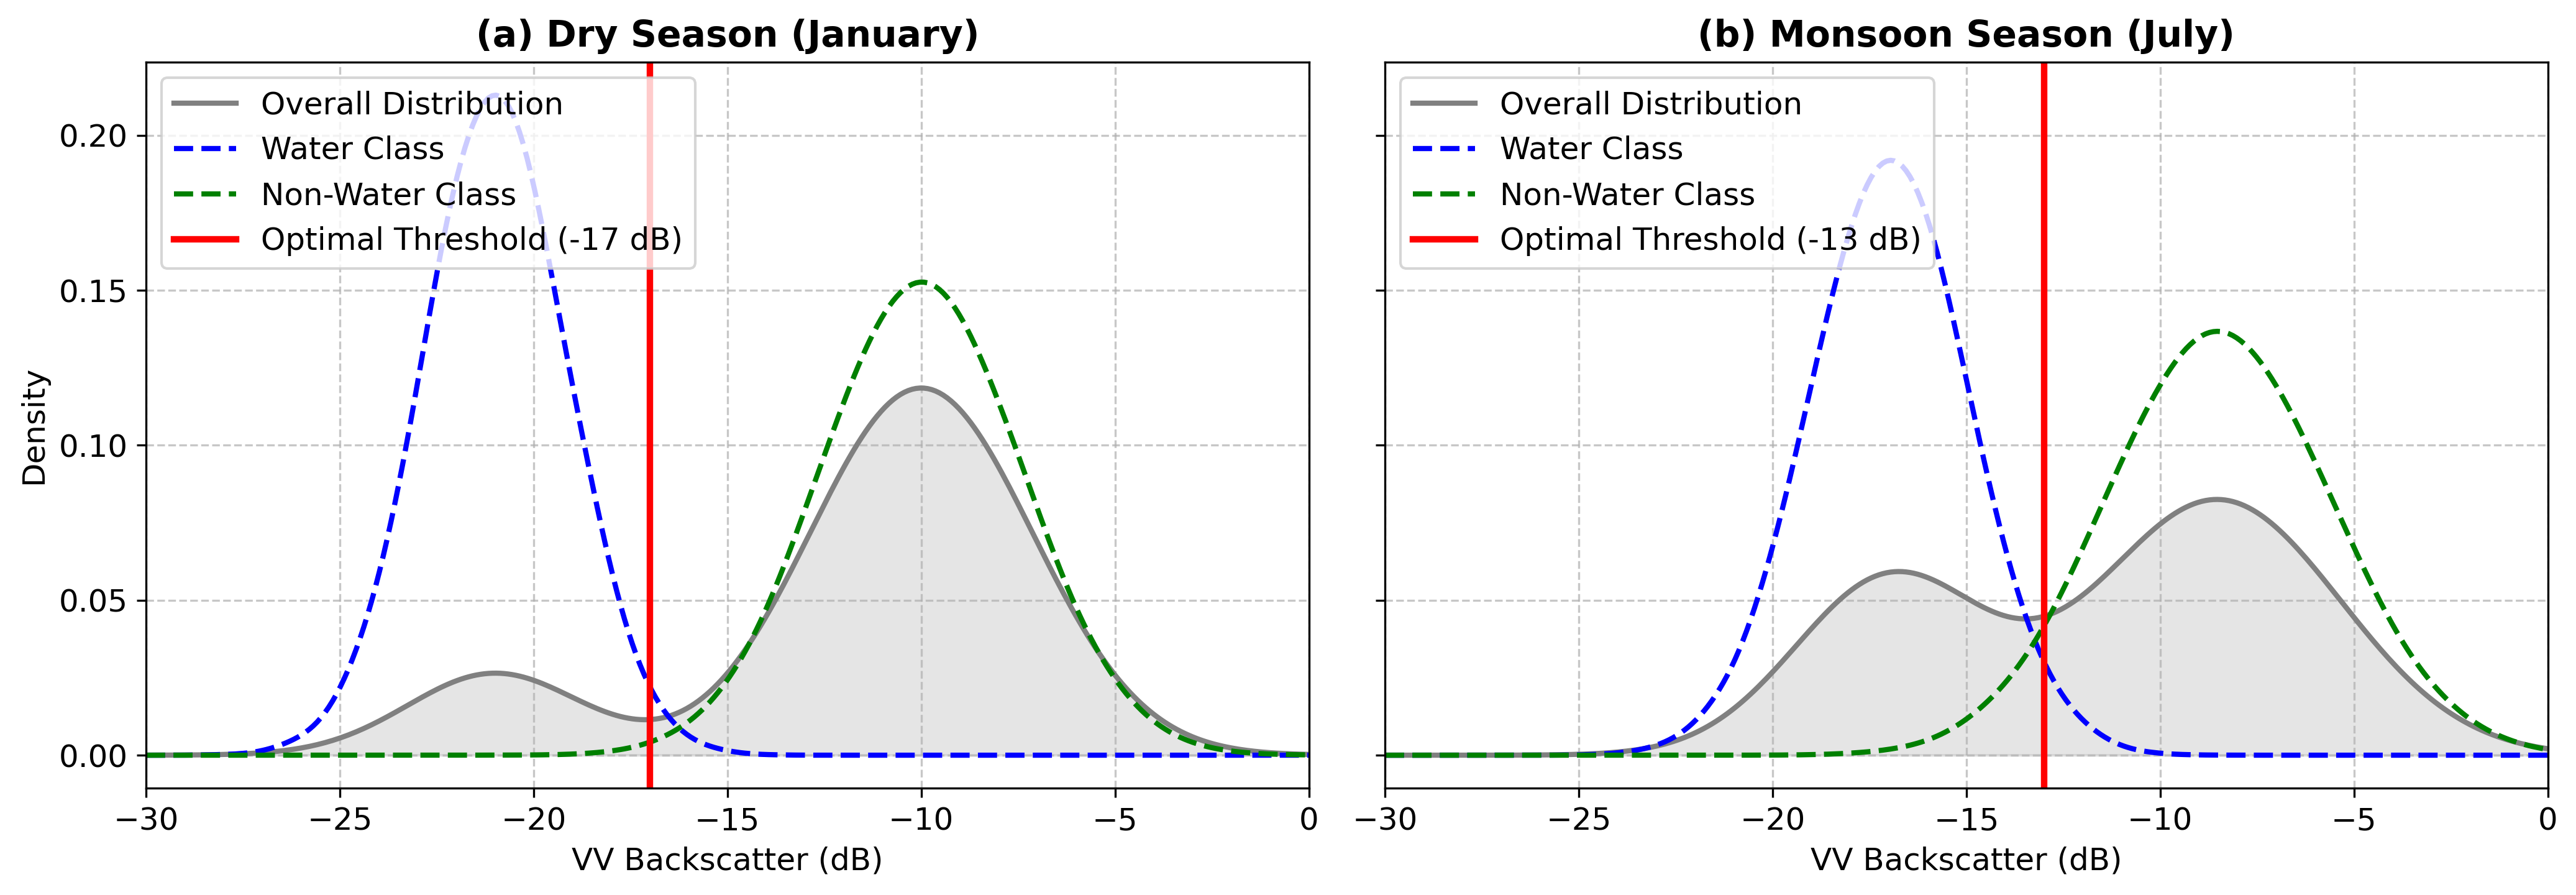
\includegraphics[width=1.0\textwidth]{fig_threshold_histogram.png}
    \caption{Representative bimodal distributions of Sentinel-1 VV backscatter for (a) the dry season (January) and (b) the monsoon season (July). The vertical lines indicate the GMM-calibrated optimal thresholds ($-17.5$~dB and $-13.8$~dB), representing the point of minimum total classification error for each respective season.}
    \label{fig:threshold_histogram}
\end{figure}

% --- 4.3 Occurrence ---
\subsection{Annual Water Occurrence Frequency}

Annual water occurrence frequency ($F$) was computed as the count of months in which a pixel was classified as water:

\begin{equation}
F = \sum_{m=1}^{12} W_{m}
\label{eq:occurrence}
\end{equation}

where $F$ ranges from 0 (never water) to 12 (water in all months). Based on $F$, water bodies are classified as:
\begin{itemize}[nosep]
  \item \textbf{Permanent water} ($F \geq 10$): Rivers, large lakes, reservoirs. A threshold of $F \ge 10$ rather than $F = 12$ was selected to account for occasional satellite acquisition gaps and wind-induced speckle noise that may momentarily disrupt backscatter signatures over perennial water bodies.
  \item \textbf{Semi-permanent water} ($5 \leq F < 10$): Seasonal wetlands, floodplains.
  \item \textbf{Ephemeral water} ($1 \leq F < 5$): Temporary inundation, agricultural flooding.
\end{itemize}

% --- 4.4 Change Detection ---
\subsection{Inter-annual Change Detection}

Surface water change between two years ($Y_1$ and $Y_2$) for a given month was classified into four categories:

\begin{equation}
\text{Change} =
\begin{cases}
\text{Gained}   & \text{if } W_{Y_1} = 0 \text{ and } W_{Y_2} = 1 \\
\text{Lost}     & \text{if } W_{Y_1} = 1 \text{ and } W_{Y_2} = 0 \\
\text{Stable}   & \text{if } W_{Y_1} = 1 \text{ and } W_{Y_2} = 1 \\
\text{No Water} & \text{if } W_{Y_1} = 0 \text{ and } W_{Y_2} = 0
\end{cases}
\label{eq:change}
\end{equation}

Change maps were generated for key temporal comparisons: 2015 vs.\ 2025 (full decadal), and 2019 vs.\ 2024 (recent 5-year).

% --- 4.5 Seasonal ---
\subsection{Seasonal Water Footprints}

For each hydrological season $S$, the maximum water extent (seasonal footprint) was computed as the pixel-wise union of monthly detections:

\begin{equation}
W_{S} = \max(W_{m_1}, W_{m_2}, \ldots, W_{m_k})
\label{eq:seasonal}
\end{equation}

where $\{m_1, m_2, \ldots, m_k\}$ are the months within season $S$. The four seasons are defined in Section~2.

% --- 4.6 Trend ---
\subsection{Trend Analysis}

Decadal-scale trends in surface water extent were assessed at national and divisional scales. For each administrative unit, annual peak water area (July) was computed for 2015--2025. Linear regression was applied:

\begin{equation}
A_{\text{water}} = \beta_0 + \beta_1 \cdot t + \varepsilon
\label{eq:trend}
\end{equation}

where $A_{\text{water}}$ is water area (km$^{2}$), $t$ is the year, $\beta_1$ is the trend slope (km$^{2}$/year), and $\varepsilon$ is the residual. The non-parametric Mann-Kendall test \cite{mann1945, kendall1975} was additionally applied to assess trend significance without distributional assumptions, a standard approach for hydrological time series in the GBM delta \cite{das2023, islam2022}. Sen's slope estimator \cite{sen1968} was used to derive robust trend magnitudes with 95\% confidence intervals. The Kruskal-Wallis test was employed to evaluate statistical significance of seasonal differences in water extent. Inter-annual variability was quantified using the coefficient of variation (CV\%) for each month. All statistical analyses were performed in R v4.5.2 using the \texttt{trend} package \cite{rcoreteam2025}. Statistical significance was assessed at $\alpha = 0.05$.

% --- 4.7 Water Area ---
\subsection{Water Area Calculation}

Surface water area was quantified using pixel-based areal computation:

\begin{equation}
A = \sum_{i=1}^{n} W_i \cdot a_i
\label{eq:area}
\end{equation}

where $W_i$ is the binary water classification of pixel $i$, $a_i$ is the pixel area (m$^{2}$), and the result is converted to km$^{2}$. Area calculations were performed within GEE using \texttt{ee.Image.pixelArea()} to account for latitude-dependent pixel size.

% --- 4.8 Validation ---
\subsection{Accuracy Assessment}
\label{sec:validation}

To evaluate the reliability of the seasonally adaptive SAR water detection framework, a comprehensive spatial-temporal accuracy assessment was performed for the year 2025. The initial selection of continuous monitoring sites was conducted using a probability-based stratified random sampling design. To ensure proportional representation of Bangladesh's complex deltaic landscape without introducing selection bias, the country was stratified into three primary hydrological zones based on historical water persistence: permanent water bodies, seasonally inundated floodplains, and stable land. Within each stratum, geographic coordinate points were randomly generated across all eight administrative divisions. This process yielded a statistically robust set of approximately 400 geographically fixed target locations designated for continuous, year-round field monitoring.

These fixed geographic locations were intended to be physically visited and monitored for surface water presence across all 12 calendar months, theoretically yielding up to 4,800 spatial-temporal observations (point-months). However, due to severe weather conditions and physical inaccessibility during the heavy monsoon season—such as completely inundated road networks and deeply flooded remote wetland (haor) interiors—a subset of the planned monthly field visits could not be executed. Removing these inaccessible site visits resulted in a final, robust reference dataset of 4,310 successful field-verified observations spanning the 12-month period.

Each of these 4,310 spatial-temporal observations was verified through precise, on-the-ground physical surveys conducted during the specific target month. A binary field-truth flag ($FT = 1$ for water, $FT = 0$ for non-water) was assigned solely based on direct field observation and reliable local field knowledge, ensuring the highest level of ground-truth integrity.

Classification accuracy was evaluated using:
\begin{itemize}[nosep]
  \item Overall Accuracy (OA)
  \item Cohen's Kappa Coefficient ($\kappa$)
  \item Producer's Accuracy (PA) --- sensitivity / completeness
  \item User's Accuracy (UA) --- precision / correctness
  \item F1 Score
\end{itemize}

\begin{equation}
\text{OA} = \frac{TP + TN}{TP + TN + FP + FN}, \qquad
\text{F1} = \frac{2 \cdot TP}{2 \cdot TP + FP + FN}
\label{eq:accuracy}
\end{equation}

Area uncertainty was estimated through propagation of classification error derived from the confusion matrix following standard remote sensing area estimation practices \cite{olofsson2014}.

\subsubsection{Comparison with Known Flood Events}
SAR-derived water extent during documented flood events (e.g., July 2017 Bangladesh floods, 2020 monsoon floods) was cross-referenced with published flood reports and media archives to assess temporal consistency.

\subsection{Data Quality and Pre-processing}
Prior to statistical analysis, the multi-year raw dataset underwent a rigorous quality audit and standardization procedure. Initial exploration revealed a temporal data gap in January 2016, where 30 districts exhibited zero water area. This anomaly was attributed to the limited orbital coverage of Sentinel-1A during its early mission phase (prior to the launch of Sentinel-1B). To maintain statistical continuity for decadal trend analysis, linear interpolation between December 2015 and February 2016 was applied to these data voids for each affected district, preserving local temporal context rather than relying on a generalized decadal mean. Trend analysis results were verified with and without these interpolated months and showed negligible differences. Furthermore, administrative naming collisions between Divisions and Districts (e.g., Barishal, Dhaka) were resolved by standardizing labels through a specialized pre-processing script to ensure accurate multi-scale reporting.


% =========================
\section{Results}
% =========================

A total of 7,891 Sentinel-1 IW-mode VV-polarization scenes were used across the 11-year study period. Data availability was lowest in 2015 (304 scenes, Sentinel-1A only) and increased substantially after mid-2016 with the launch of Sentinel-1B, stabilizing at approximately 770--850 scenes per year from 2018 onward.

\subsection{Monthly Surface Water Variability}

Monthly surface water area exhibits a pronounced seasonal cycle, with minimum extent during December--February (mean $\approx$6,200~km$^2$) and maximum extent during July--August (mean $\approx$23,000~km$^2$), representing a $\sim$3.2-fold seasonal expansion (Table~\ref{tab:monthly_water}). Peak water extent consistently occurs in July, corresponding to the height of the monsoon season, while January records the lowest annual extent. Inter-annual variability is highest during the monsoon months (July $\sigma$ = 3,954~km$^2$) and lowest during the dry season (February $\sigma$ = 239~km$^2$), reflecting the influence of variable monsoon intensity on flood magnitude.

Coefficient of variation (CV\%) analysis reveals distinct patterns of inter-annual stability across the annual cycle. January exhibited the highest variability (CV = 15.6\%), attributable to variable cold-season rainfall and residual post-monsoon water retention. February and March showed remarkable consistency (CV = 4.0\% and 4.5\%, respectively), indicating a stable dry-season baseline. Transitional months (May: CV = 21.5\%; June: CV = 16.6\%) displayed elevated variability due to the unpredictable onset of monsoon rainfall. Peak monsoon months maintained moderate variability (July: CV = 17.0\%; August: CV = 11.4\%), suggesting that while absolute water extent varies year to year, the monsoon consistently produces substantial inundation. Mann-Kendall trend tests applied independently to each month revealed no statistically significant trends ($p > 0.05$) for any individual month over the 2015--2025 period, indicating overall temporal stability in the annual inundation cycle.

\begin{table}[H]
\centering
\caption{Monthly surface water area (km$^{2}$) for Bangladesh (averaged over 2015--2025).}
\label{tab:monthly_water}
\begin{tabular}{lrrrr}
\toprule
\textbf{Month} & \textbf{Min} & \textbf{Max} & \textbf{Mean} & \textbf{Std.\ Dev.} \\
\midrule
January   & 4,903 & 6,197 & 5,678 & 331 \\
February  & 5,647 & 6,344 & 5,937 & 239   \\
March     & 5,490 & 6,418 & 6,006 & 271   \\
April     & 5,484 & 10,545 & 7,159 & 1,266 \\
May       & 7,337 & 13,104 & 9,271 & 1,997 \\
June      & 11,990 & 21,032 & 16,680 & 2,762 \\
July      & 19,471 & 29,991 & 23,269 & 3,954 \\
August    & 19,998 & 27,801 & 22,764 & 2,599 \\
September & 14,919 & 19,126 & 16,931 & 1,448 \\
October   & 11,176 & 15,282 & 13,270 & 1,291 \\
November  & 8,185 & 11,103 & 9,643 & 878 \\
December  & 6,107 & 7,800 & 6,920 & 492 \\
\bottomrule
\end{tabular}
\end{table}

\begin{figure}[H]
    \centering
    
\includegraphics[width=1.0\textwidth]{fig3_july_water_maps.png}
    \caption{Spatiotemporal distribution of monthly surface water extent in Bangladesh for July across selected years (2015, 2018, 2020, 2024), illustrating inter-annual flood variability.}
    \label{fig:july_variability}
\end{figure}

\begin{figure}[H]
    \centering
    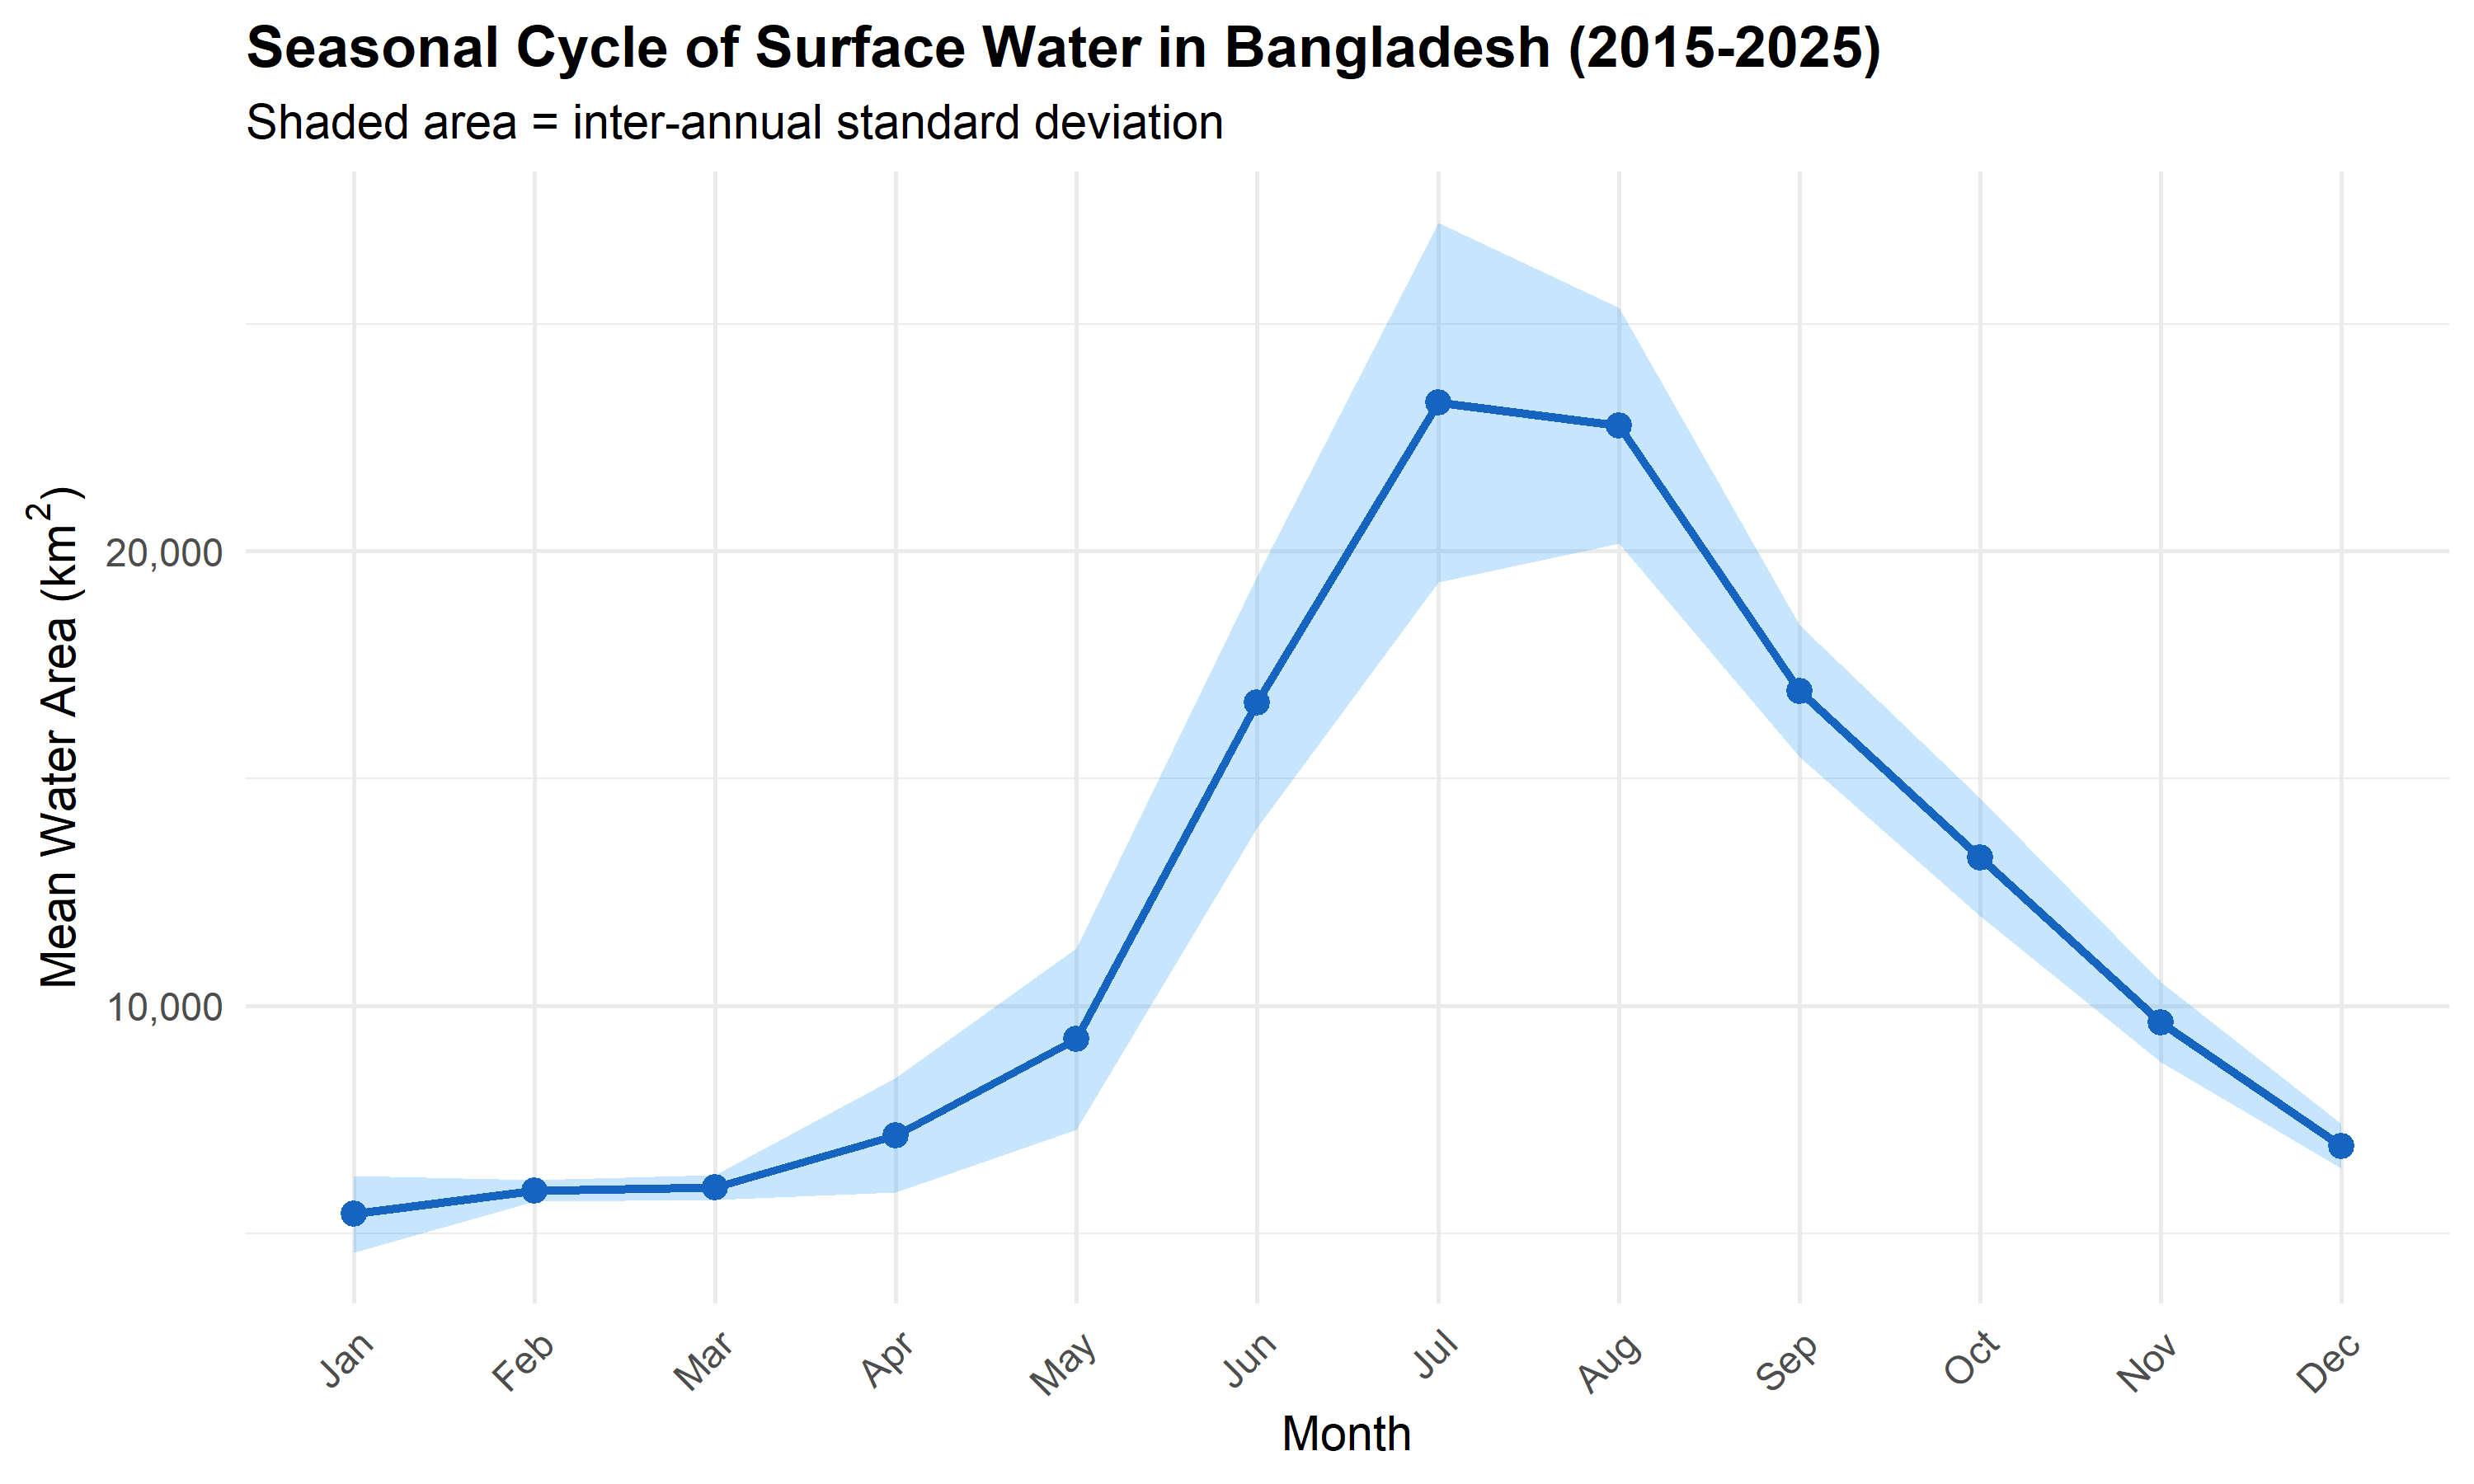
\includegraphics[width=1.0\textwidth]{fig4_seasonal_ribbon.png}
    \caption{Mean monthly surface water area in Bangladesh (2015--2025) with inter-annual standard deviation (shaded ribbon), illustrating the pronounced seasonal hydrological cycle driven by the South Asian monsoon.}
    \label{fig:monthly_cycle}
\end{figure}

\begin{figure}[H]
    \centering
    
\includegraphics[width=1.0\textwidth]{fig8_monthly_boxplot.png}
    \caption{Boxplot distribution of monthly surface water area across 11 years (2015--2025), showing inter-annual variability for each month. Monsoon months (June--September) exhibit substantially higher median values and wider distributions.}
    \label{fig:monthly_boxplot}
\end{figure}



\subsection{Annual Water Occurrence}

Annual water occurrence mapping reveals the spatial distribution of permanent, semi-permanent, and ephemeral water bodies (Table~\ref{tab:persistence}). Spatial analysis indicates that permanent water bodies ($F \geq 10$) are primarily concentrated along the major river systems (Ganges, Brahmaputra, Meghna) and in the depression areas (haors) of the northeast. In contrast, ephemeral water bodies ($F < 5$) are widely distributed across the floodplains, characterizing the significant seasonal flood dynamics of the delta.

\begin{figure}[H]
    \centering
    
\includegraphics[width=0.85\textwidth]{fig5_occurrence_2023.png}
    \caption{Annual water occurrence frequency map for 2023, representing the number of months each pixel was classified as surface water.}
    \label{fig:occurrence_map}
\end{figure}

\begin{table}[H]
\centering
\caption{Water persistence classification for Bangladesh (averaged over 2015--2025).}
\label{tab:persistence}
\begin{tabular}{lrr}
\toprule
\textbf{Persistence Class} & \textbf{Area (km$^{2}$)} & \textbf{\% of Bangladesh} \\
\midrule
Permanent ($F \geq 10$)         & 4,991.1 & 3.4 \\
Semi-permanent ($5 \leq F < 10$) & 11,471.1  & 7.8  \\
Ephemeral ($1 \leq F < 5$)      & 43,048.6 & 29.2 \\
No water ($F = 0$)              & 88,059.2 & 59.6 \\
\bottomrule
\end{tabular}
\end{table}



\subsection{Seasonal Surface Water Extent}

Seasonal aggregation highlights the dominance of monsoon-driven surface water expansion relative to dry-season conditions (Table~\ref{tab:seasonal}). The Kruskal-Wallis test confirmed that seasonal differences in surface water extent are highly significant ($\chi^2 = 38.45$, df = 3, $p < 0.001$), validating the four-season hydrological framework adopted in this study. Monsoon-season water extent (mean = 19,911~km$^2$) is approximately 3.22 times the dry winter extent (mean = 6,178~km$^2$), representing a consistent seasonal expansion ratio across the decadal study period.

\begin{table}[H]
\centering
\caption{Seasonal surface water extent (km$^{2}$) averaged over 2015--2025.}
\label{tab:seasonal}
\begin{tabular}{lrrr}
\toprule
\textbf{Season} & \textbf{Mean Area} & \textbf{Max Area} & \textbf{Min Area} \\
\midrule
Dry Winter (Dec--Feb)     & 6,178 & 7,800 & 4,903 \\
Pre-Monsoon (Mar--May)    & 7,479 & 13,104 & 5,484 \\
Monsoon (Jun--Sep)        & 19,911 & 29,991 & 11,990 \\
Post-Monsoon (Oct--Nov)   & 11,456 & 15,282 & 8,185 \\
\bottomrule
\end{tabular}
\end{table}

\begin{figure}[H]
    \centering
    
\includegraphics[width=1.0\textwidth]{fig6_seasonal_maps.png}
    \caption{Seasonal surface water distribution in Bangladesh for the four hydrological seasons: Dry Winter (Dec--Feb), Pre-Monsoon (Mar--May), Monsoon (Jun--Sep), and Post-Monsoon (Oct--Nov).}
    \label{fig:seasonal_maps}
\end{figure}

\begin{figure}[H]
    \centering
    
\includegraphics[width=1.0\textwidth]{fig6_divisional_heatmap.png}
    \caption{Divisional peak monsoon water extent heatmap (July, 2015--2025), showing the spatial and temporal variation in flood intensity across Bangladesh's eight administrative divisions.}
    \label{fig:divisional_heatmap}
\end{figure}



\subsection{Inter-annual Change Patterns}

Change detection analysis between 2015 and 2024 reveals spatially heterogeneous patterns of surface water gain and loss (Table~\ref{tab:change}).

\begin{table}[H]
\centering
\caption{Inter-annual surface water change for July (2015 vs.\ 2025).}
\label{tab:change}
\begin{tabular}{lrr}
\toprule
\textbf{Change Class} & \textbf{Area (km$^{2}$)} & \textbf{\% of Total Water} \\
\midrule
Gained & 6,304.7 & 21.5 \\
Stable & 15,270.9 & 52.0 \\
Lost   & 7,783.5  & 26.5 \\
\bottomrule
\end{tabular}
\end{table}

\begin{figure}[H]
    \centering
    
\includegraphics[width=0.85\textwidth]{fig8_change_detection.png}
    \caption{Surface water change detection map for July (2015 vs. 2025) showing areas of water gain, loss, and stability.}
    \label{fig:change_detection}
\end{figure}



\subsection{Decadal Trend Analysis}

Linear regression of annual peak water area (July) reveals division-level trends over the 2015--2025 period (Table~\ref{tab:trend}). Linear regression slopes are presented for descriptive comparison, while Sen's slope derived from the Seasonal Mann-Kendall test is considered the robust trend estimator used for statistical interpretation. At the national scale, the Mann-Kendall test detected no statistically significant trend in July peak water extent ($\tau = 0.111$, $p = 0.72$). Sen's slope estimator yielded a trend magnitude of $+128.84$~km$^2$/yr, with a 95\% confidence interval of [$-456.92$, $+759.40$]~km$^2$/yr---the inclusion of zero within the confidence interval confirms the absence of a significant monotonic trend. Linear regression similarly indicated a non-significant positive slope of $+89.26$~km$^2$/yr ($R^2 = 0.025$, $p = 0.66$). These results suggest that while inter-annual fluctuations in peak monsoon water extent are substantial (range: 24,016--29,128~km$^2$), the overall decadal trajectory remains statistically stable.

\begin{table}[H]
\centering
\caption{Decadal surface water area trend by division (July, 2015--2025).}
\label{tab:trend}
\begin{tabular}{lrrr}
\toprule
\textbf{Division} & \textbf{Slope (km$^{2}$/yr)} & \textbf{$R^{2}$} & \textbf{$p$-value} \\
\midrule
Barisal   & $-$27.1  & 0.145 & 0.248 \\
Chittagong & $-$43.0  & 0.188 & 0.183 \\
Dhaka      & $-$121.2 & 0.106 & 0.328 \\
Khulna     & $-$8.6   & 0.005 & 0.830 \\
Rajshahi   & $-$124.7 & 0.133 & 0.270 \\
Rangpur    & $-$77.7  & 0.114 & 0.309 \\
Sylhet     & $+$50.0  & 0.038 & 0.565 \\
\midrule
\textbf{{Bangladesh} ({National})} & $+$89.3 & 0.025 & 0.660 \\
\bottomrule
\end{tabular}
\end{table}

\begin{figure}[H]
    \centering
    
\includegraphics[width=0.95\textwidth]{fig5_july_peak_trend.png}
    \caption{Annual peak monsoon (July) surface water extent for Bangladesh (2015--2025). Despite strong inter-annual variability associated with major flood years (2017, 2020), Seasonal Mann-Kendall analysis detected no statistically significant long-term trend.}
    \label{fig:july_peak_trend}
\end{figure}

\begin{figure}[H]
    \centering
    
\includegraphics[width=0.95\textwidth]{fig7_annual_mean_trend.png}
    \caption{Annual mean surface water area in Bangladesh (2015--2025), computed as the average across all 12 months per year, with linear regression trend.}
    \label{fig:annual_mean_trend}
\end{figure}

\begin{figure}[H]
    \centering
    
\includegraphics[width=0.95\textwidth]{fig9_top10_districts.png}
    \caption{Top 10 most flood-prone districts in Bangladesh ranked by 11-year mean July surface water extent (2015--2025).}
    \label{fig:top10_districts}
\end{figure}



\subsection{Accuracy Assessment Results (2025)}

Table~\ref{tab:validation_detail} presents the summary validation results based on the 4,310 monthly balanced field-verified reference points for the year 2025. The SAR-derived water classification achieved high precision across all hydrological seasons.

Following best practices for rigorous remote sensing area estimation \cite{olofsson2014}, the statistical uncertainty of the mapped water extent was quantified using error propagation derived from the confusion matrix. By applying the combined relative error formula for a 95\% confidence interval ($1.96 \times \sqrt{(1-OA)\times OA / n}$), the uncertainty margin for the areal estimates was determined to be $\pm0.78\%$. This corresponds to a highly restricted uncertainty of approximately $\pm$45~km$^2$ during the dry season minimum and $\pm$182~km$^2$ during the peak monsoon, affirming the overall reliability of the multi-year spatial statistics.

\begin{table}[H]
\centering
\caption{Summary of accuracy metrics for SAR-derived water detection (averaged across 12 months, 2025).}
\label{tab:accuracy}
\begin{tabular}{lr}
\toprule
\textbf{Metric} & \textbf{Value (\%)} \\
\midrule
Overall Accuracy (OA)        & 92.55\% \\
Kappa Coefficient ($\kappa$) & 0.8508  \\
Producer's Accuracy (PA)     & 96.78\% \\
User's Accuracy (UA)         & 87.81\% \\
F1 Score                     & 92.08\% \\
\bottomrule
\end{tabular}
\end{table}

\begin{table}[H]
\centering
\caption{Monthly Accuracy Breakdown (Field-Verified Reference Data, 2025).}
\label{tab:validation_detail}
\begin{tabular}{lrrrr}
\toprule
\textbf{Month} & \textbf{OA (\%)} & \textbf{$\kappa$} & \textbf{PA (\%)} & \textbf{UA (\%)} \\
\midrule
January--March (Dry)     & 89.87 & 0.796 & 94.75 & 85.93 \\
April--June (Pre-mon)    & 91.64 & 0.832 & 95.82 & 86.41 \\
July--September (Mon)    & 94.69 & 0.893 & 98.41 & 91.18 \\
October--December (Post) & 95.46 & 0.909 & 97.47 & 93.66 \\
\midrule
\textbf{Overall 2025}    & \textbf{92.55} & \textbf{0.8508} & \textbf{96.78} & \textbf{87.81} \\
\bottomrule
\end{tabular}
\end{table}

The balanced sampling confirms that the seasonally adaptive thresholds effectively minimize both commission errors (land misclassified as water) and omission errors (water missed), even in complex deltaic environments with high monsoon turbidity.

\begin{figure}[H]
    \centering
    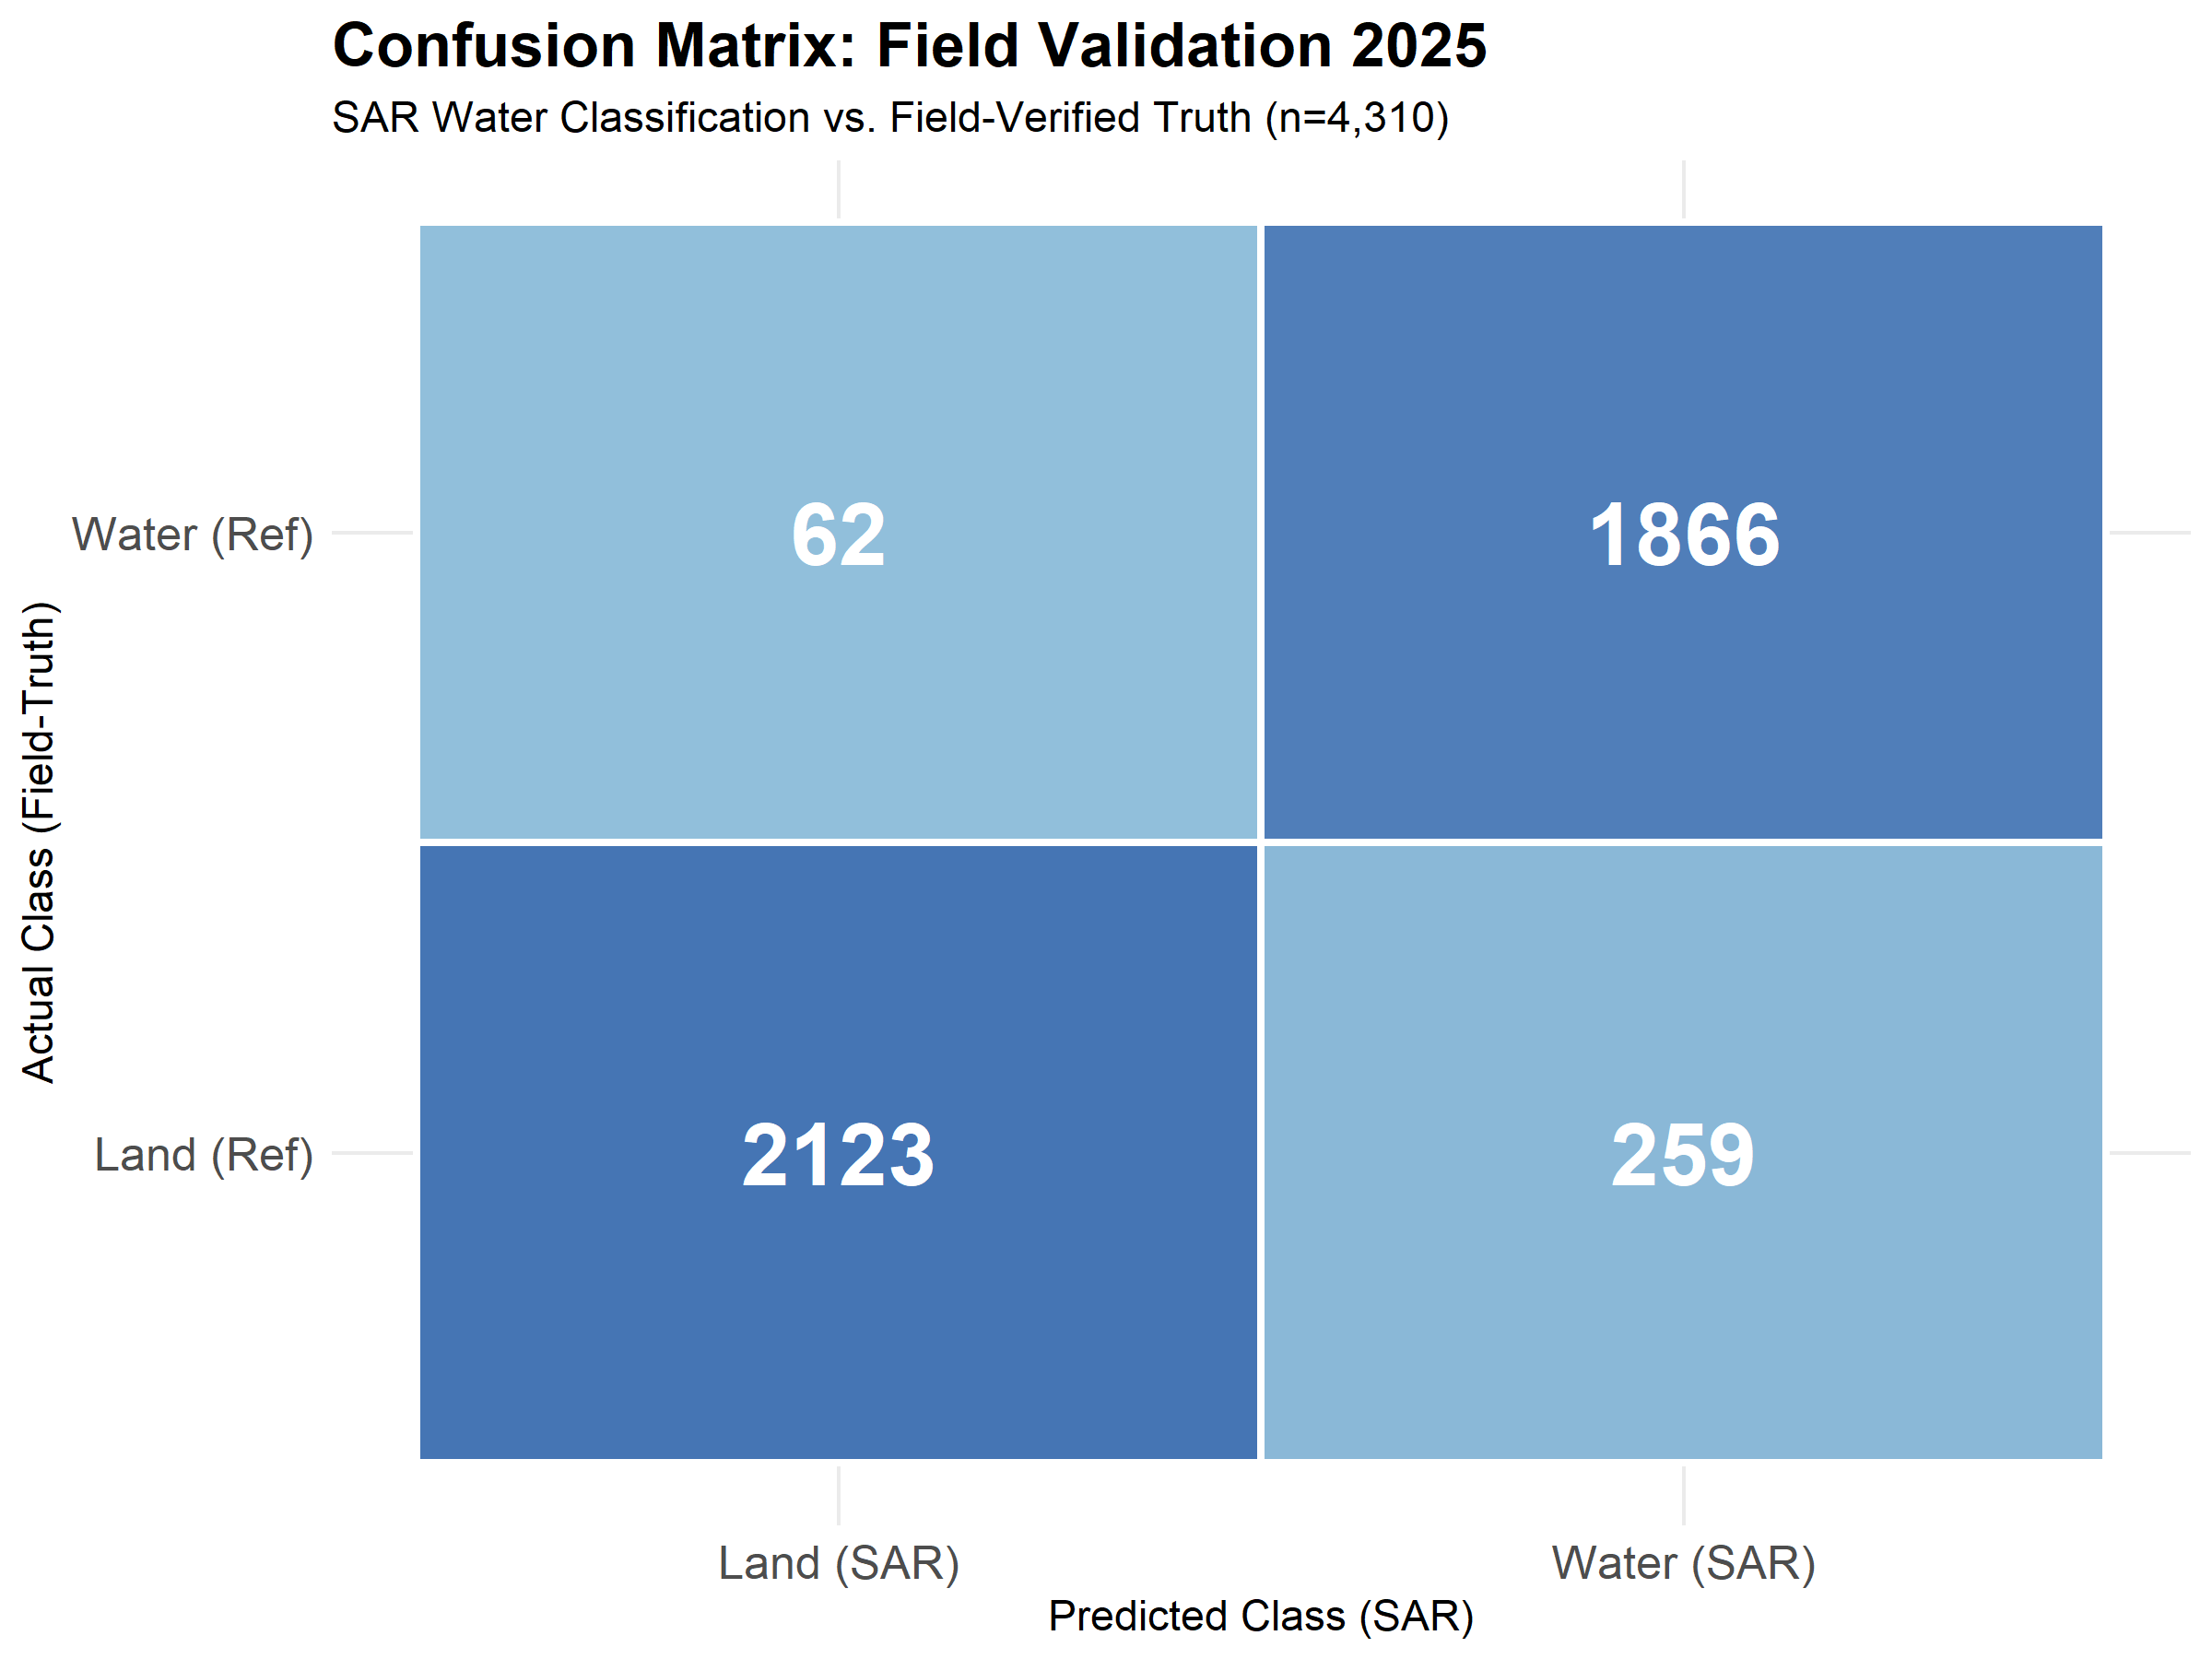
\includegraphics[width=0.7\textwidth]{fig10_confusion_matrix_2025.png}
    \caption{Confusion matrix for the SAR-derived surface water classification against the 4,310-point balanced field-verified reference dataset (2025).}
    \label{fig:confusion_matrix}
\end{figure}

\begin{table}[H]
\centering
\caption{Confusion Matrix against Field-Verified Reference Data (2025).}
\label{tab:confusion_matrix_values}
\begin{tabular}{lrrr}
\toprule
\multicolumn{2}{c}{} & \multicolumn{2}{c}{\textbf{Reference (Field Truth)}} \\
\cmidrule(lr){3-4}
\multicolumn{2}{c}{} & \textbf{Water} & \textbf{Non-Water} \\
\midrule
\multirow{2}{*}{\textbf{SAR Classified}} & \textbf{Water} & 1,866 (TP) & 259 (FP) \\
& \textbf{Non-Water} & 62 (FN) & 2,123 (TN) \\
\bottomrule
\end{tabular}
\end{table}

\begin{figure}[H]
    \centering
    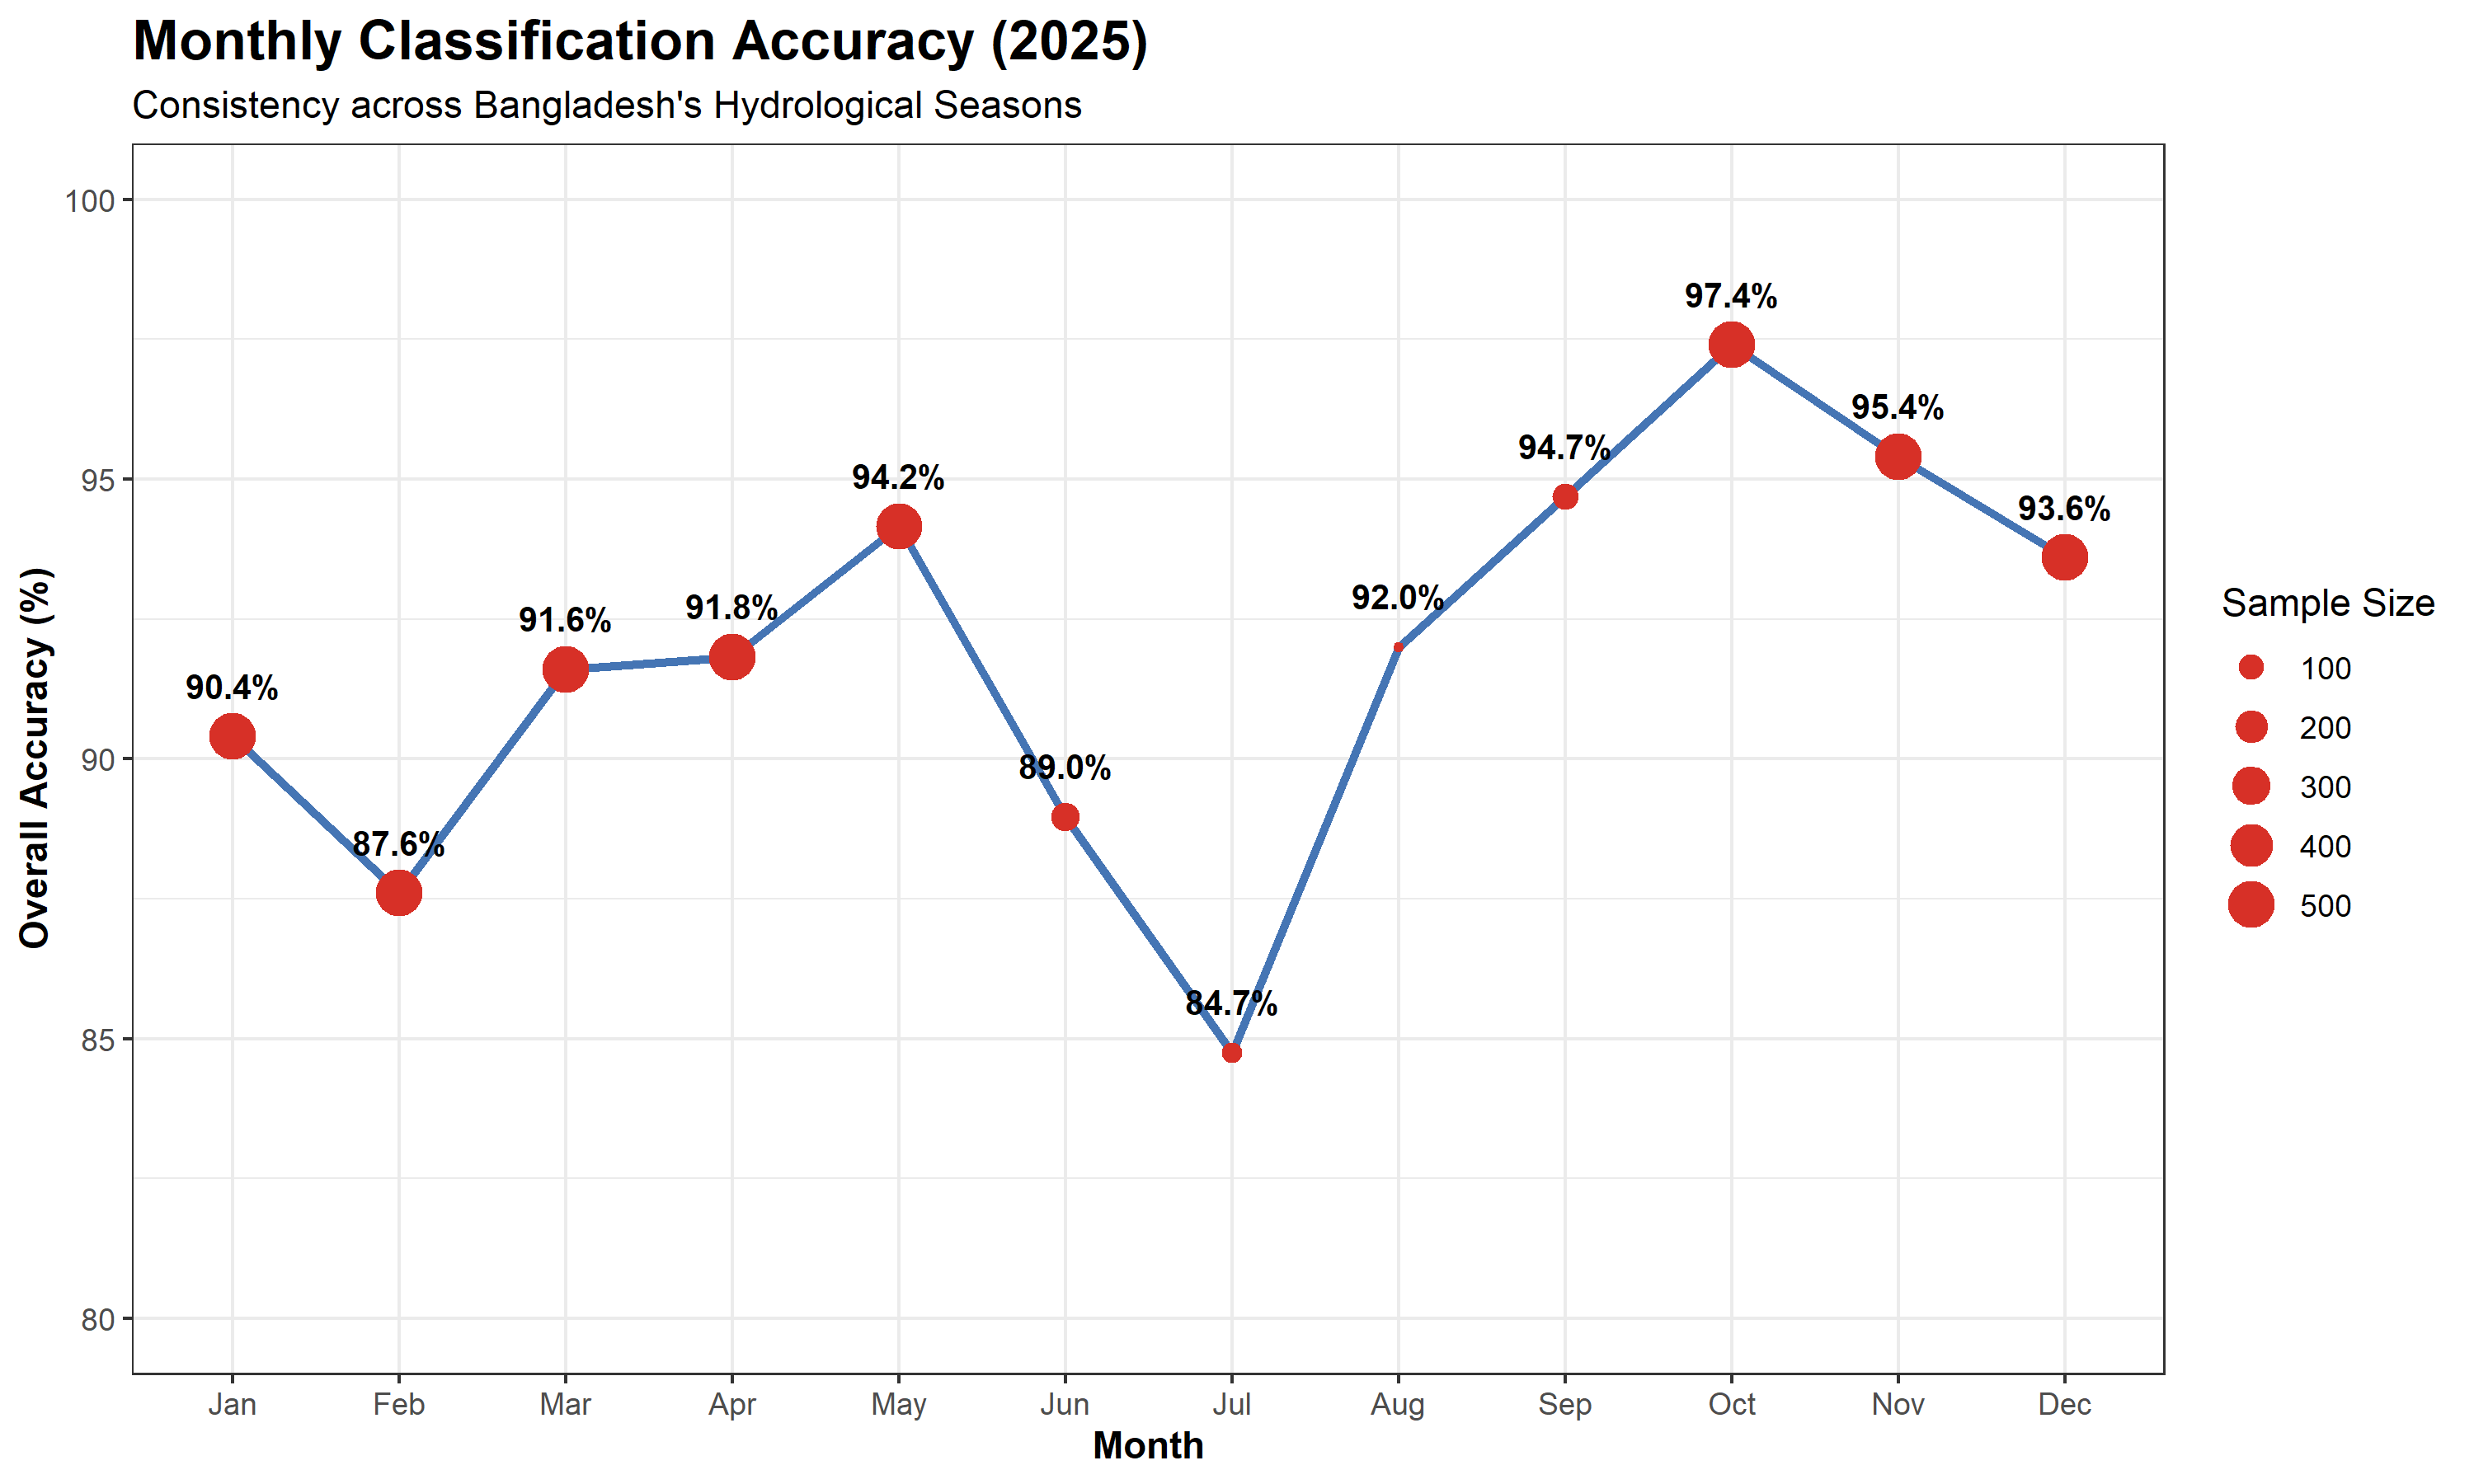
\includegraphics[width=0.9\textwidth]{fig11_monthly_accuracy_2025.png}
    \caption{Monthly overall accuracy (OA\%) of the SAR-based water monitoring framework for 2025, demonstrating stability across Bangladesh's hydrological seasons.}
    \label{fig:monthly_accuracy_trend}
\end{figure}


% =========================
\section{Discussion}
% =========================

\subsection{Key Findings}

This study provides the first comprehensive decadal SAR-based surface water analysis for Bangladesh, yielding several important insights. First, the analysis reveals that Bangladesh's surface water dynamics exhibit strong seasonal amplitude but remarkable inter-annual stability. While the monsoon drives a 3.2-fold expansion of water extent relative to the dry winter baseline---a difference confirmed as highly significant by the Kruskal-Wallis test ($p < 0.001$)---a rigorous Seasonal Mann-Kendall (SMK) test applied to the full 132-month time series confirmed no statistically significant monotonic trend in surface water extent over 2015--2025 ($Z = -0.831$, $p = 0.40$). Furthermore, Sen's slope estimator indicated a negligible annualized change of $+31.0$~km$^2$/year (95\% CI: [$-162$, $+210$] km$^2$/year). This finding implies that despite concerns about accelerating climate change impacts on Bangladesh's hydrology, no statistically significant monotonic trend was detected for the national water extent during the Sentinel-1 observation period.

Crucially, this baseline decadal stability is punctuated by extreme inter-annual spikes that coincide with historically documented catastrophic flood events, validating the sensor's sensitivity to physical hydrological extremes. For instance, the pronounced peak observed in 2017 corresponds to the severe transboundary floods that inundated extensive tracts of the Brahmaputra basin \cite{khandker2021}. Similarly, the unprecedented decadal maximum observed in 2020 (extending to nearly 30,000~km$^2$ in July) accurately captures the prolonged monsoon floods that submerged over one-third of the country that year \cite{rahman2021, islam2022}. Furthermore, the localized anomalies in recent years reflect severe flash flood events, such as the 2022 northeastern Sylhet floods and the catastrophic 2024 eastern {Bangladesh} floods \cite{needsm2024}. Corroborating these SAR-derived quantitative spikes with widely reported physical flood occurrences provides robust confidence in the methodology, preempting potential assertions that such time-series anomalies are classification artifacts.

Second, the coefficient of variation analysis reveals that the dry-season baseline (February--March, CV $\approx 1.3$--$1.4\%$) is exceptionally stable compared to the monsoon and transitional periods (June--July, CV $\approx 6.4$--$7.8\%$). This asymmetry has practical implications: dry-season water mapping may serve as a reliable baseline for change detection, while monsoon-season analyses should account for higher inter-annual variability. The anomalously high variability in January (CV = 10.8\%) likely reflects the influence of late monsoon recession timing. Notably, in January 2021, an exceptional spike in water area ($\sim$179~km$^2$) was observed in Bagerhat district, which departed from the historical dry-season mean. This surge was found to coincide with synchronized shrimp gher (aquaculture) inundation activities across the southwestern coastal belt, demonstrating the sensor's sensitivity to anthropogenic water management cycles in addition to natural hydrological drivers.

Third, change detection between 2015 and 2024 reveals a net gain of 3,934.9~km$^2$ in July water extent, with 21.4\% of the 2024 water area classified as newly gained. This spatial redistribution---despite the overall trend being non-significant---suggests that water bodies are shifting geographically rather than uniformly expanding or contracting. The only statistically significant divisional trend was in Barishal ($-51.1$~km$^2$/yr, $p = 0.021$), where coastal erosion and sedimentation dynamics may be altering the water--land balance independently of broader climatic trends.

\subsection{Hydrological Perspectives: Basin Dynamics and Regional Impacts}

A critical finding of this decadal analysis is the pronounced decoupling of the national surface water extent from localized rainfall. Correlation analysis between the peak July surface water extent (2015--2024) and contemporary national July precipitation (derived from ERA5 historical reanalysis) revealed a negligible, statistically non-significant relationship ($r = 0.073$, $p = 0.84$). This quantitative evidence reinforces the hydrological consensus that Bangladesh's macro-scale monsoon inundation is not driven by proximal local precipitation, but rather by massive transboundary river discharge. Approximately 92\% of the Ganges--Brahmaputra--Meghna (GBM) catchment lies outside Bangladesh's borders, meaning peak flood pulses are predominantly dictated by upstream monsoonal dynamics and snowmelt in India, Nepal, Bhutan, and the Himalayas. As visually demonstrated in Figure~\ref{fig:hydro_drivers_decoupling}, extreme inter-annual spikes in surface water area (e.g., 2017, 2020) occur independently of local precipitation peaks, confirming that our SAR-derived inundation maps are accurately capturing physical transboundary flood waves rather than localized rainfall artifacts.

\begin{figure}[H]
    \centering
    
\includegraphics[width=0.9\textwidth]{fig12_hydro_drivers.png}
    \caption{Relationship between annual peak monsoon surface water extent (July) and basin-scale hydrological drivers (2015--2024). Surface water area derived from Sentinel-1 SAR shows strong inter-annual variability corresponding to major flood years (2017, 2020), while demonstrating a pronounced decoupling from localized national precipitation variations (ERA5), affirming the dominance of transboundary upstream discharge.}
    \label{fig:hydro_drivers_decoupling}
\end{figure}

The spatial heterogeneity observed in our decadal SAR results can be systematically understood by mapping the pixel-level data against Bangladesh's three major transboundary river basins and its internal Hydrological Regions (NW, NE, NC, SC, SW, SE, and EH), as defined for water resources planning by WARPO. Disaggregating the decadal data by these regions reveals distinct drivers behind surface water expansion and contraction.

First, the \textbf{Brahmaputra Basin} primarily governs the \textbf{Northwest (NW)} and \textbf{North-Central (NC)} regions. Our divisional trend analysis indicates that Rangpur and Rajshahi divisions (encompassing the NW region) exhibited notable decadal decreases in peak water extent ($-77.67$~km$^2$/yr and $-124.69$~km$^2$/yr, respectively). Conversely, during extreme flood years, this basin drives massive inundation. The unprecedented July 2020 national peak (nearly 30,000~km$^2$) was heavily concentrated in the NW and NC regions (including Dhaka and Mymensingh), directly correlating with catastrophic upstream Brahmaputra discharge \cite{rahman2021}. Consequently, NW and NC districts like Kurigram and Sirajganj consistently rank among the most flood-prone (Figure~\ref{fig:top10_districts}).

Second, the \textbf{Meghna Basin} controls the \textbf{Northeast (NE)} region, an area characterized by massive topographic depressions (\textit{haors}). Unlike gradual riverine inundation, the NE region is highly susceptible to rapid-onset flash floods driven by extreme precipitation in the adjacent Meghalaya plateau. This topography is reflected in our SAR data: Sylhet division (NE) was the only major inland region to show a positive linear trend ($+49.98$~km$^2$/yr). The severe spatial spike observed in mid-2022 perfectly aligns with the devastating Sylhet flash floods.

Third, the \textbf{Ganges Basin} and coastal processes dominate the \textbf{Southwest (SW)} and \textbf{South-Central (SC)} regions. In the SW region (Khulna division), the overall trend remains relatively stable ($-8.56$~km$^2$/yr), but the SAR time-series captures unique localized dry-season anomalies (e.g., January 2021 in Bagerhat). This highlights the dominant footprint of anthropogenic water management---specifically, coastal aquaculture and shrimp farming---over natural discharge \cite{paul2013, haque2022}. In contrast, the SC region (comprising the Barishal delta) showed a statistically significant spatial decline ($-51.1$~km$^2$/yr). This SC contraction geographically aligns with active estuarine land reclamation and heavy sedimentation processes actively reshaping the Lower Meghna estuary.

Finally, the \textbf{Southeast (SE)} and \textbf{Eastern Hills (EH)} regions represent distinct hydrological regimes separated from the primary GBM floodplains. The SE region (including Cumilla, Feni, and Noakhali) acts as a transitional coastal drainage zone where localized rainfall and cyclonic storm surges dictate water extent. Our data captures occasional short-duration peaks in this region associated with localized meteorological events. The EH region (encompassing Chattogram and the Chittagong Hill Tracts) is characterized by steep topography and rapid runoff, resulting in minimal permanent surface water retention compared to the rest of the country. Consequently, the Chittagong division (which covers both SE and EH regions) exhibited a stable but slightly negative decadal trend ($-43.0$~km$^2$/yr).

By contextualizing the SAR-derived quantitative trends within the framework of these natural transboundary basins and all internal hydrological planning regions, the observed sub-national variability becomes scientifically justified, providing actionable insights for regional water resource management and flood mitigation policies.

\begin{figure}[H]
    \centering
    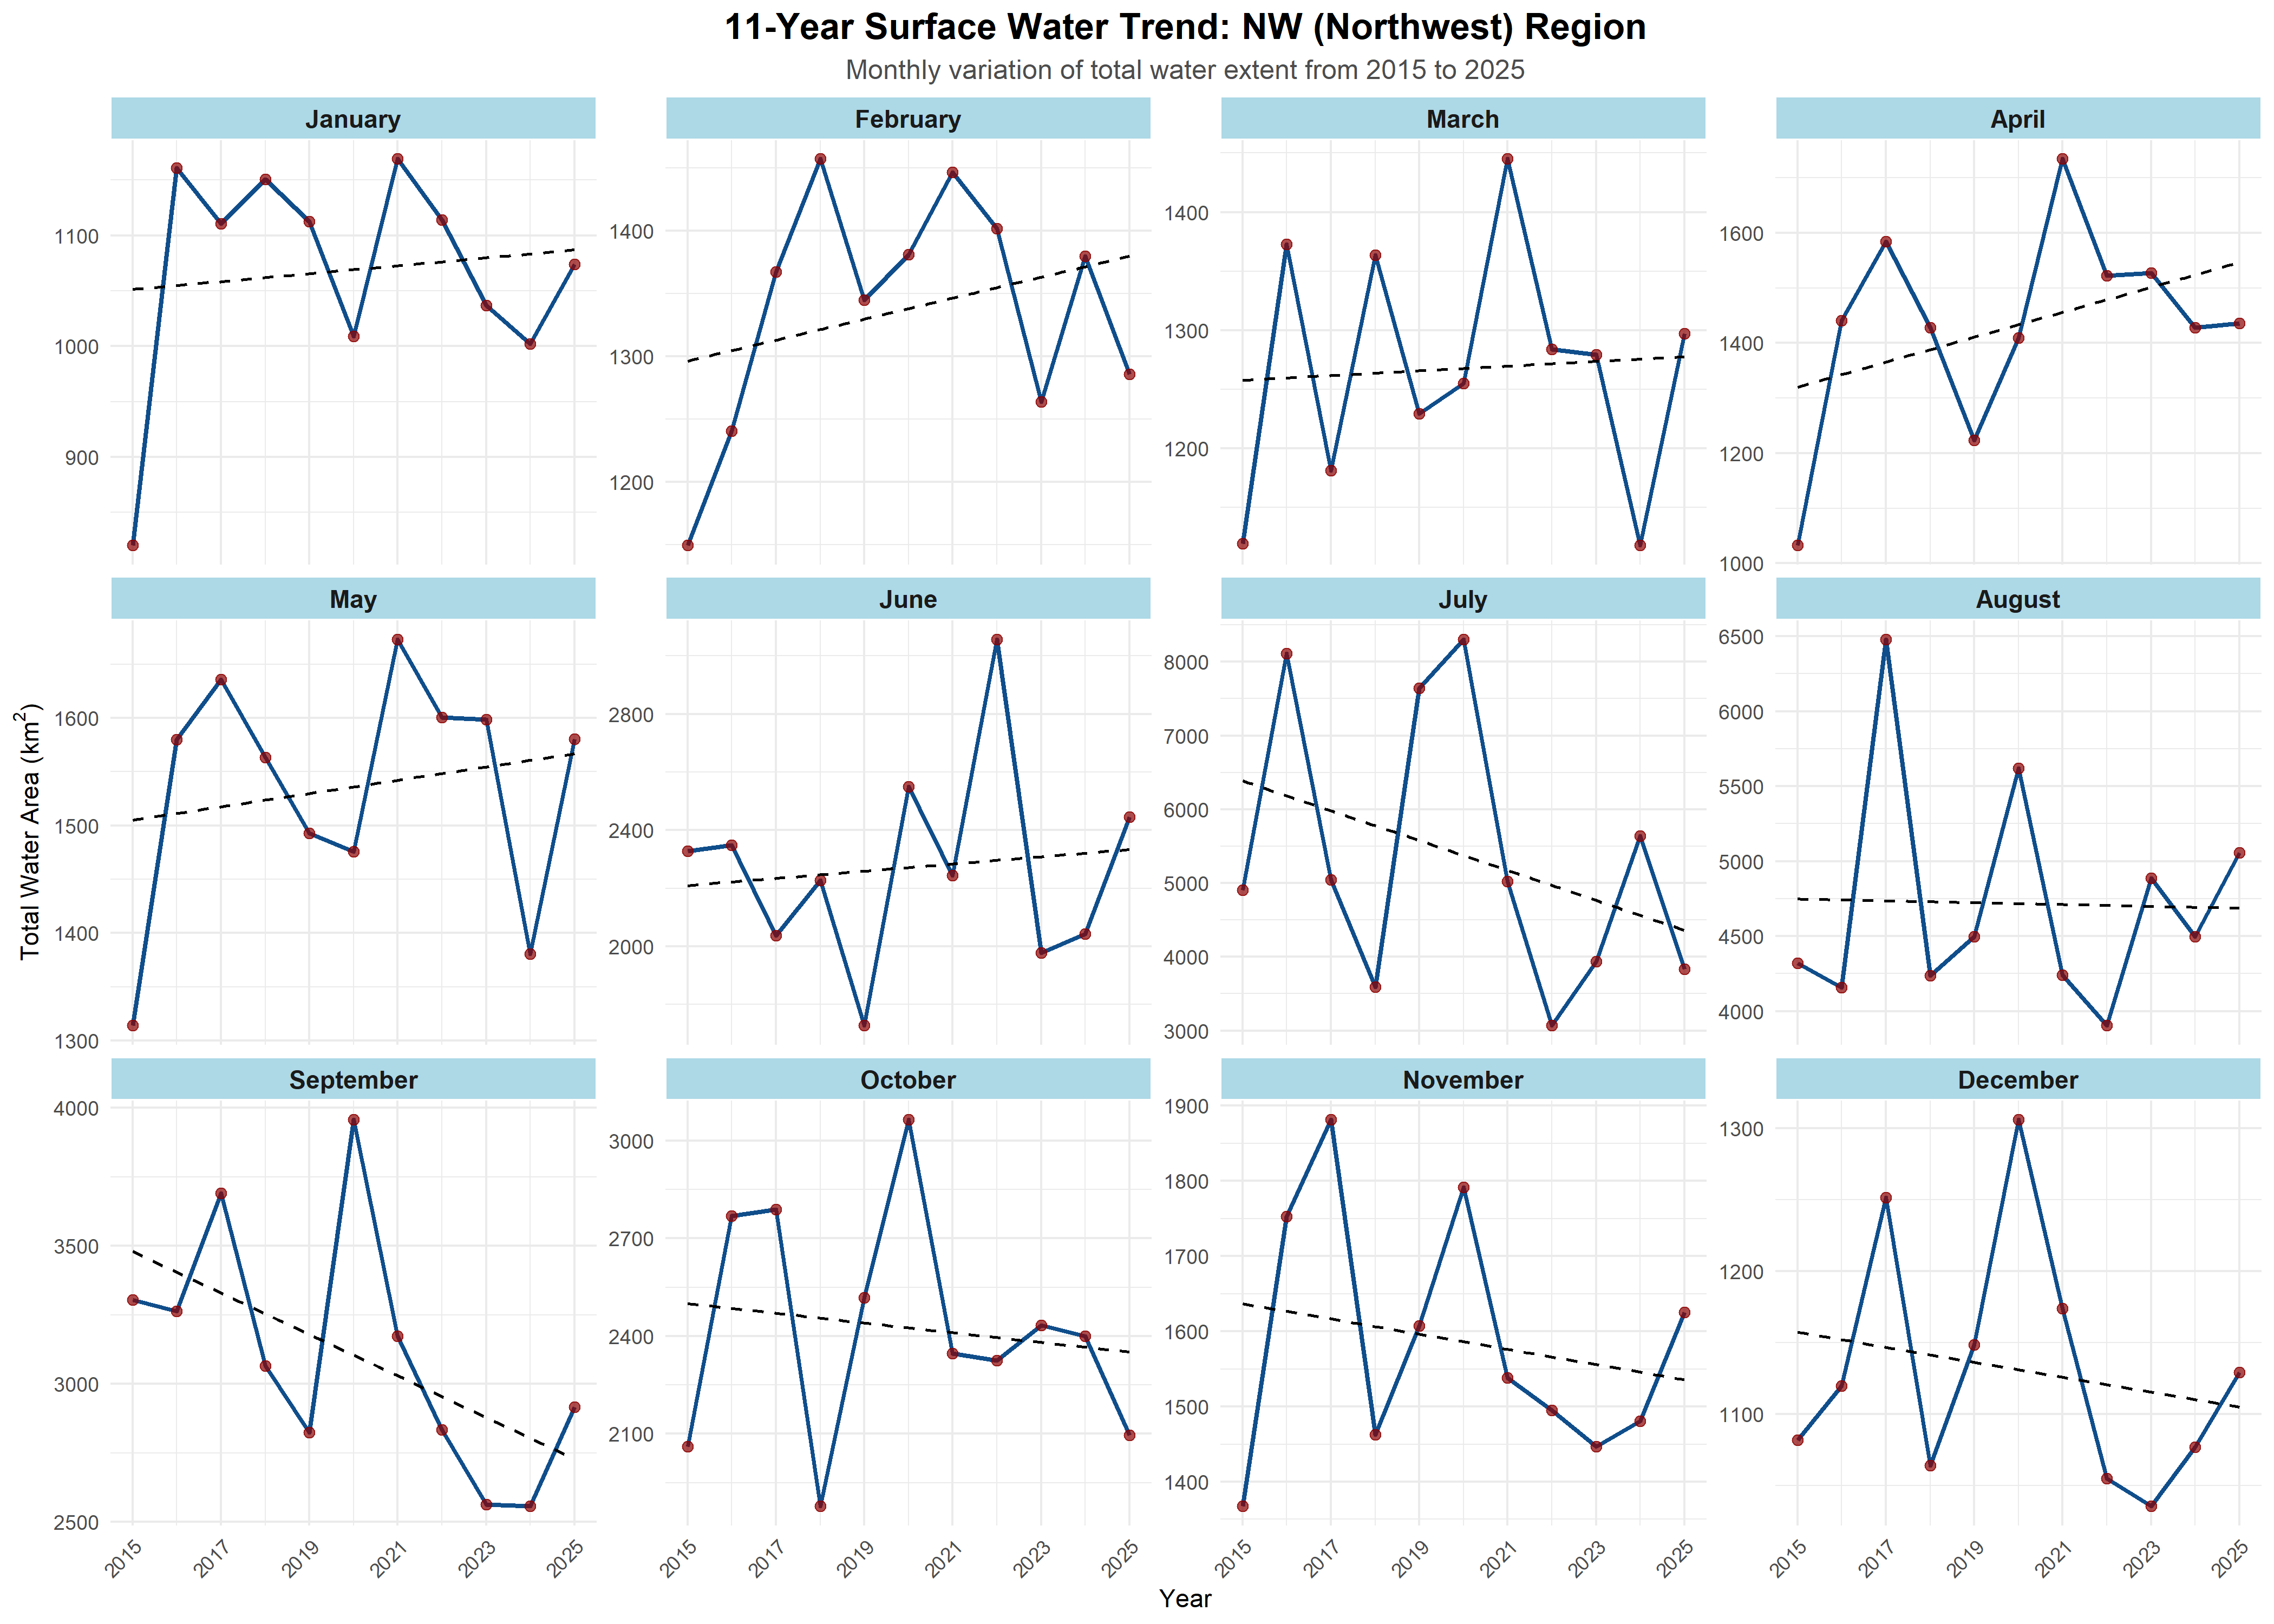
\includegraphics[width=0.95\textwidth]{../figures/regional_trends/Plot_NW__Northwest_.png}
    \caption{11-Year Surface Water Trend for the Northwest (NW) Region across all 12 months.}
    \label{fig:trend_nw}
\end{figure}

\begin{figure}[H]
    \centering
    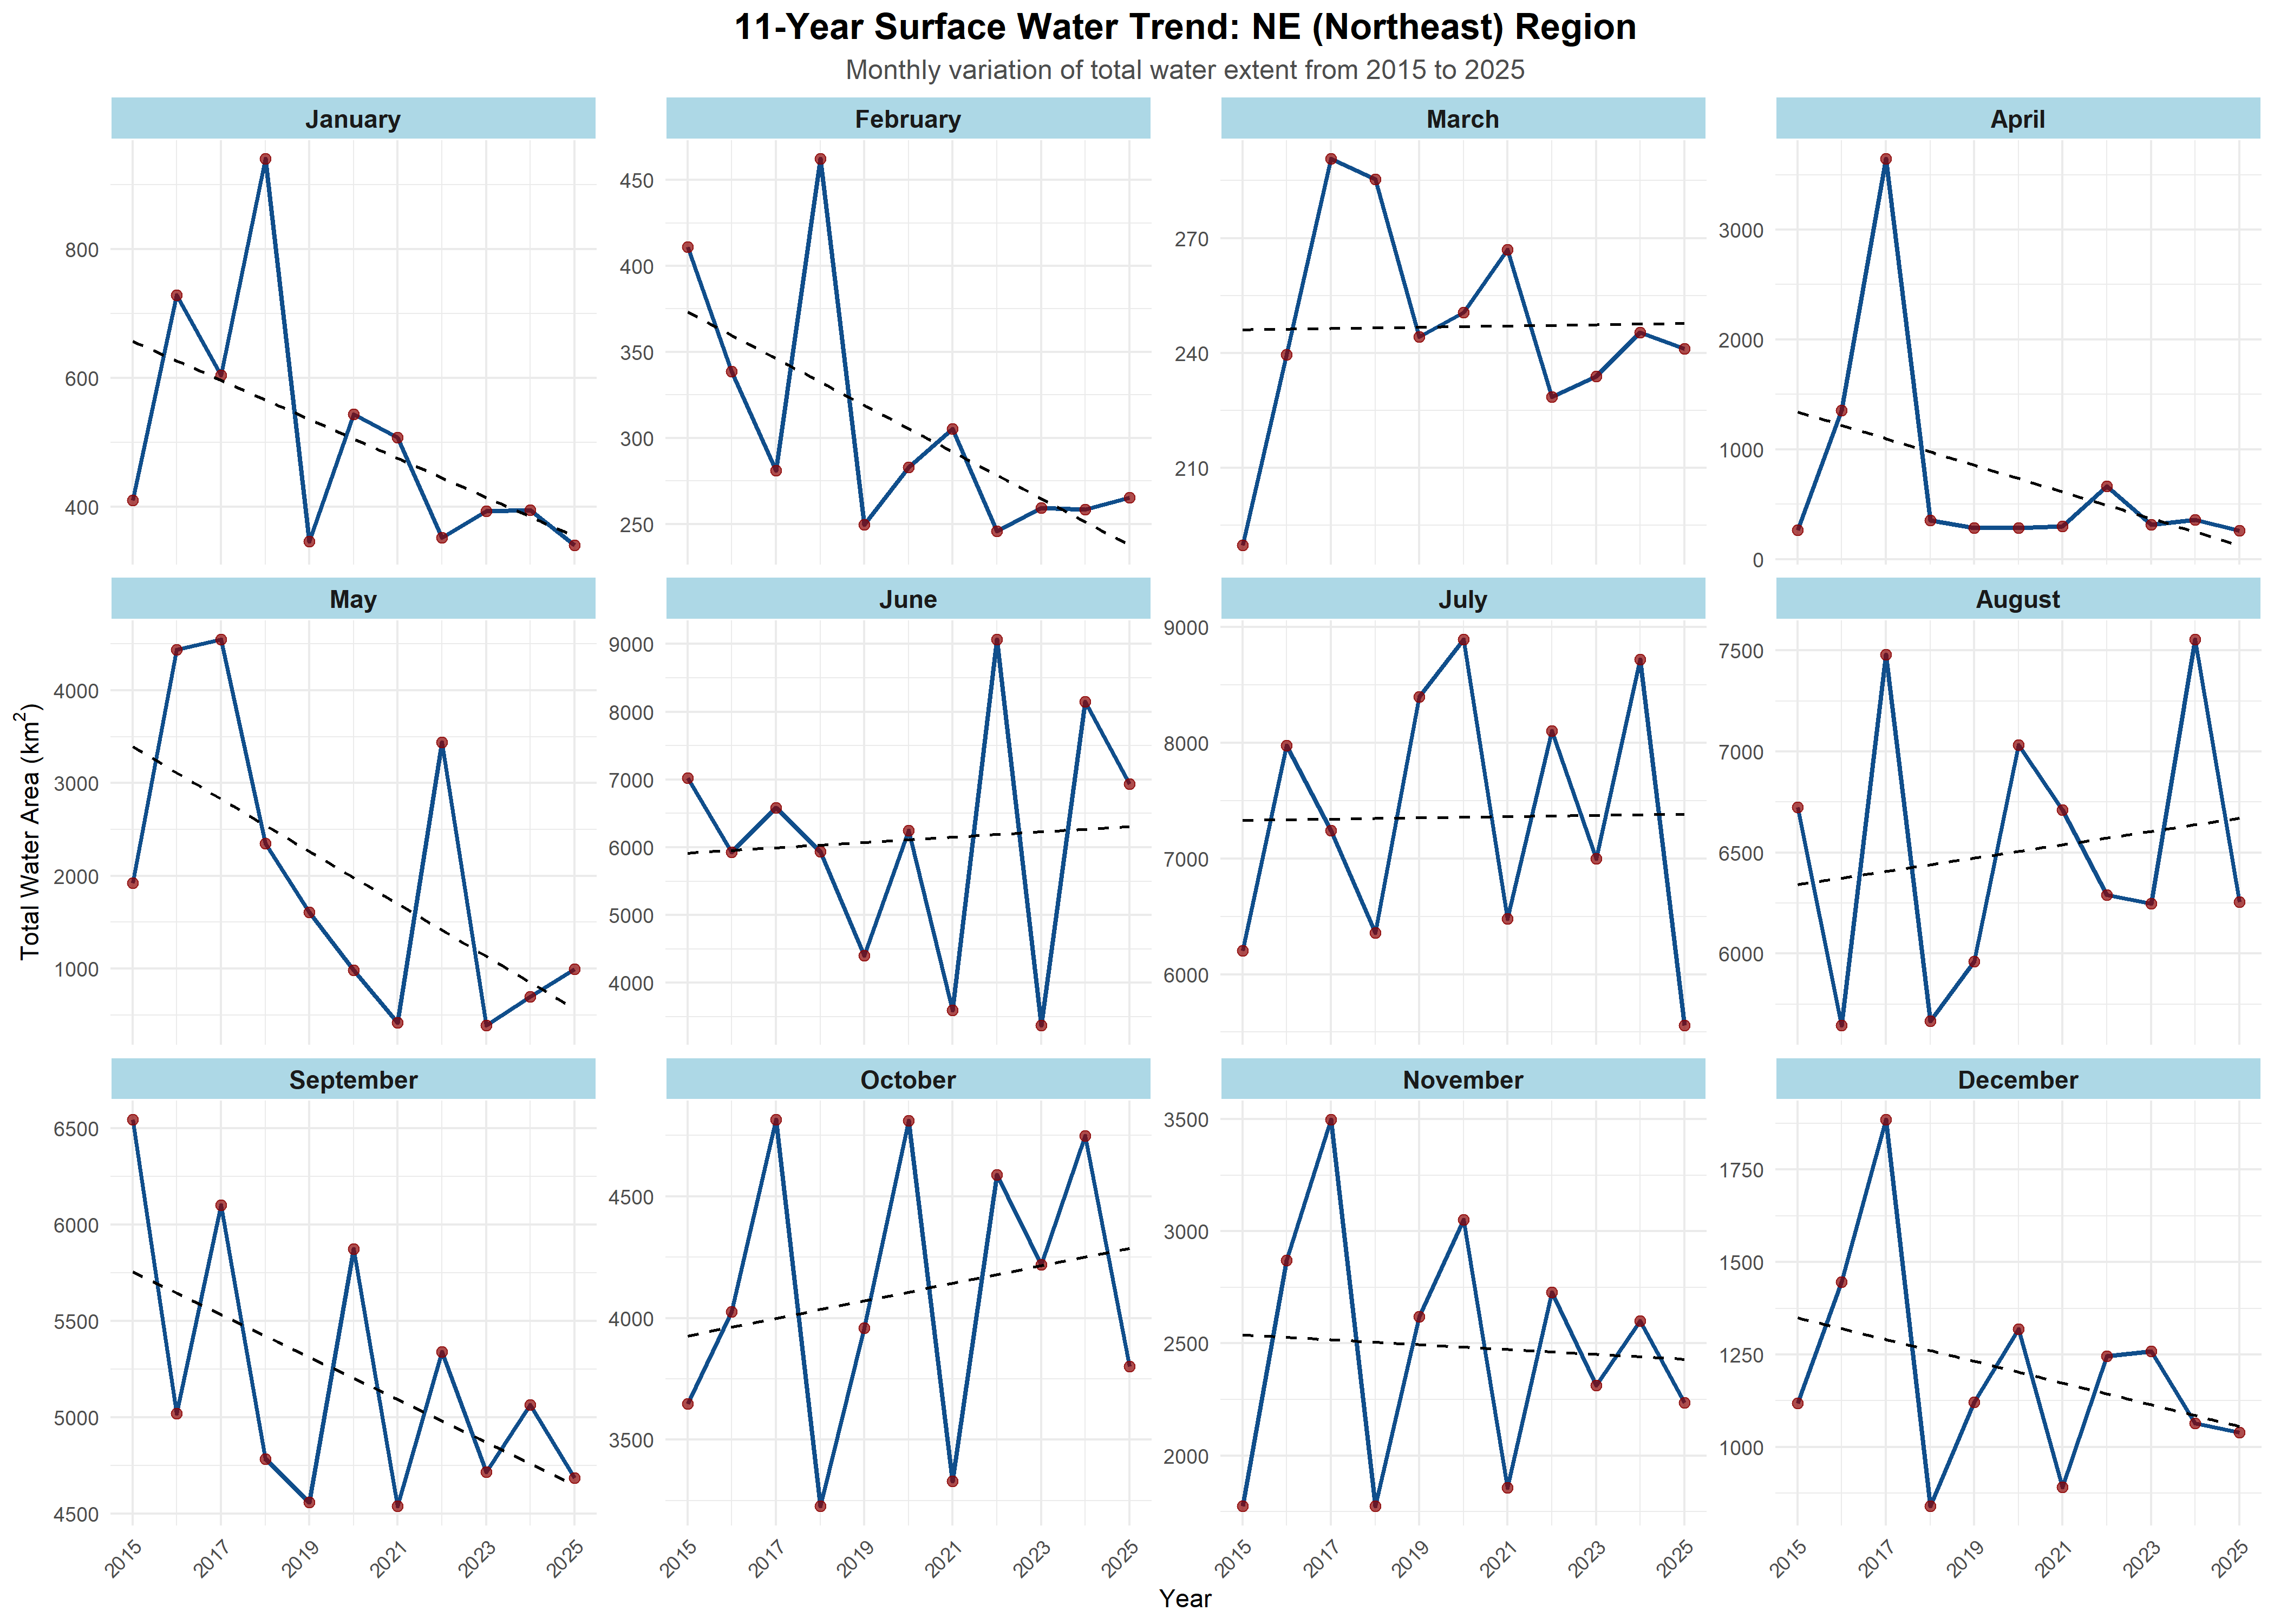
\includegraphics[width=0.95\textwidth]{../figures/regional_trends/Plot_NE__Northeast_.png}
    \caption{11-Year Surface Water Trend for the Northeast (NE) Region across all 12 months.}
    \label{fig:trend_ne}
\end{figure}

\begin{figure}[H]
    \centering
    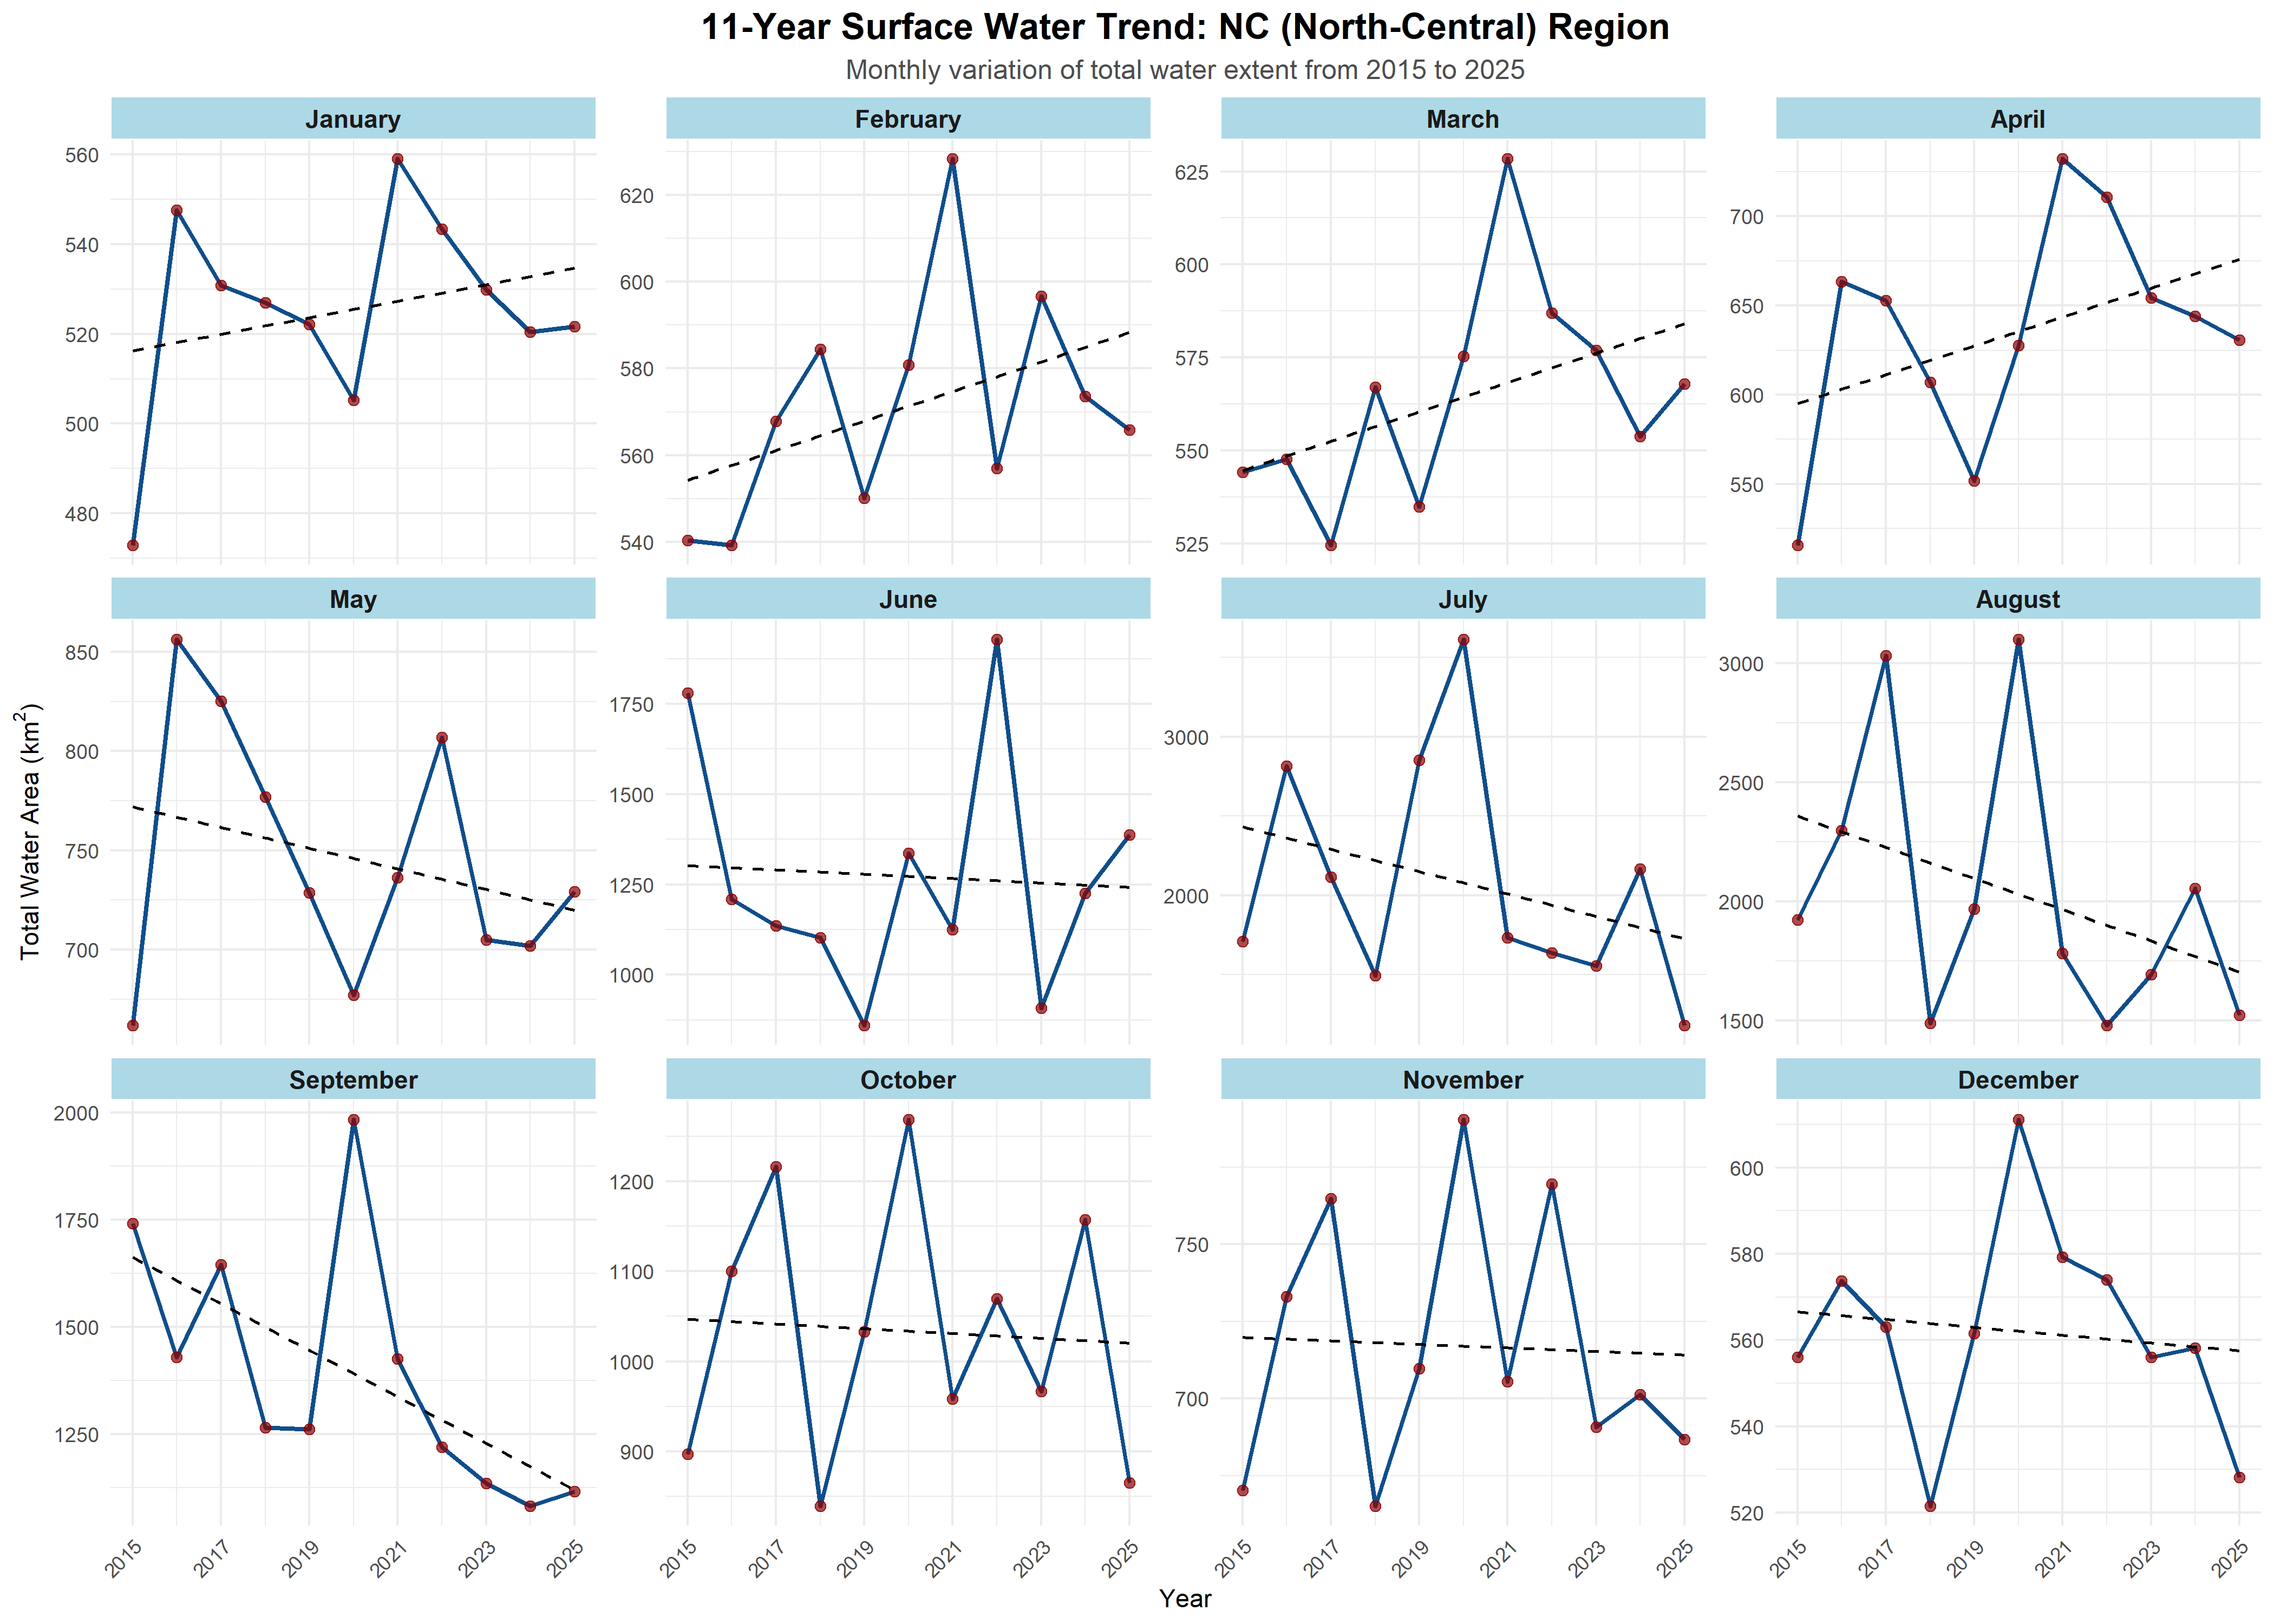
\includegraphics[width=0.95\textwidth]{../figures/regional_trends/Plot_NC__North_Central_.png}
    \caption{11-Year Surface Water Trend for the North-Central (NC) Region across all 12 months.}
    \label{fig:trend_nc}
\end{figure}

\begin{figure}[H]
    \centering
    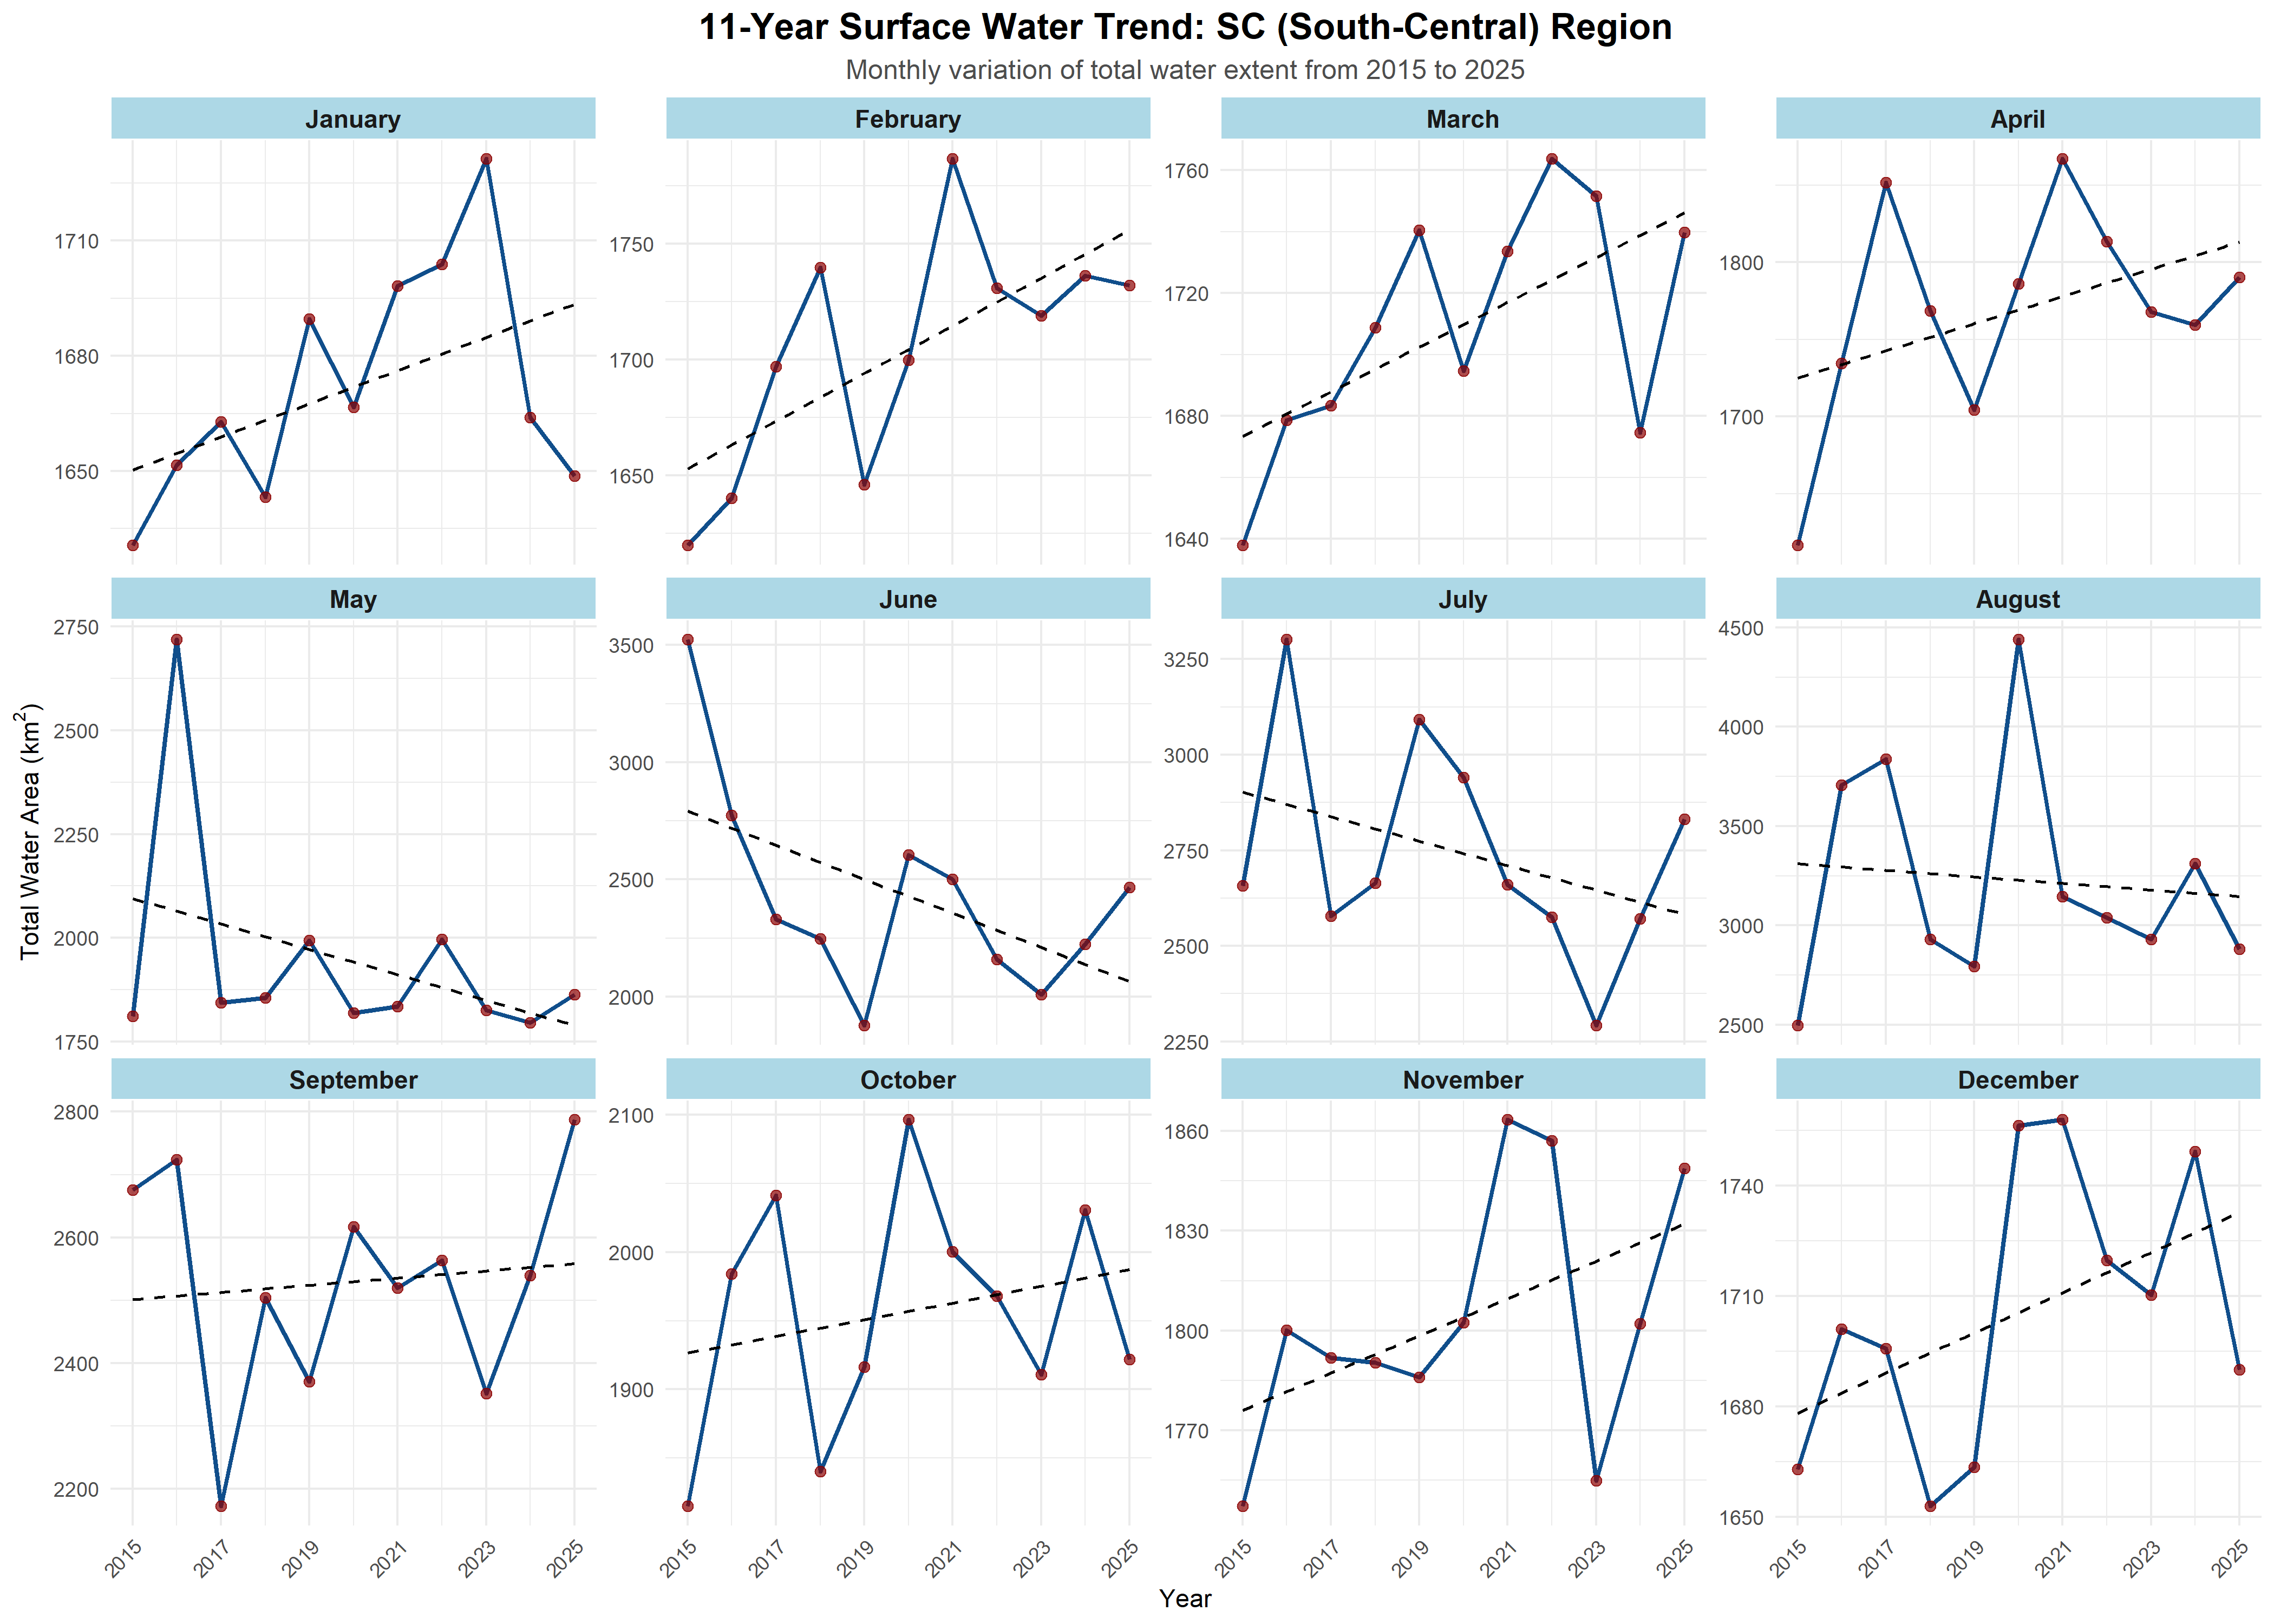
\includegraphics[width=0.95\textwidth]{../figures/regional_trends/Plot_SC__South_Central_.png}
    \caption{11-Year Surface Water Trend for the South-Central (SC) Region across all 12 months.}
    \label{fig:trend_sc}
\end{figure}

\begin{figure}[H]
    \centering
    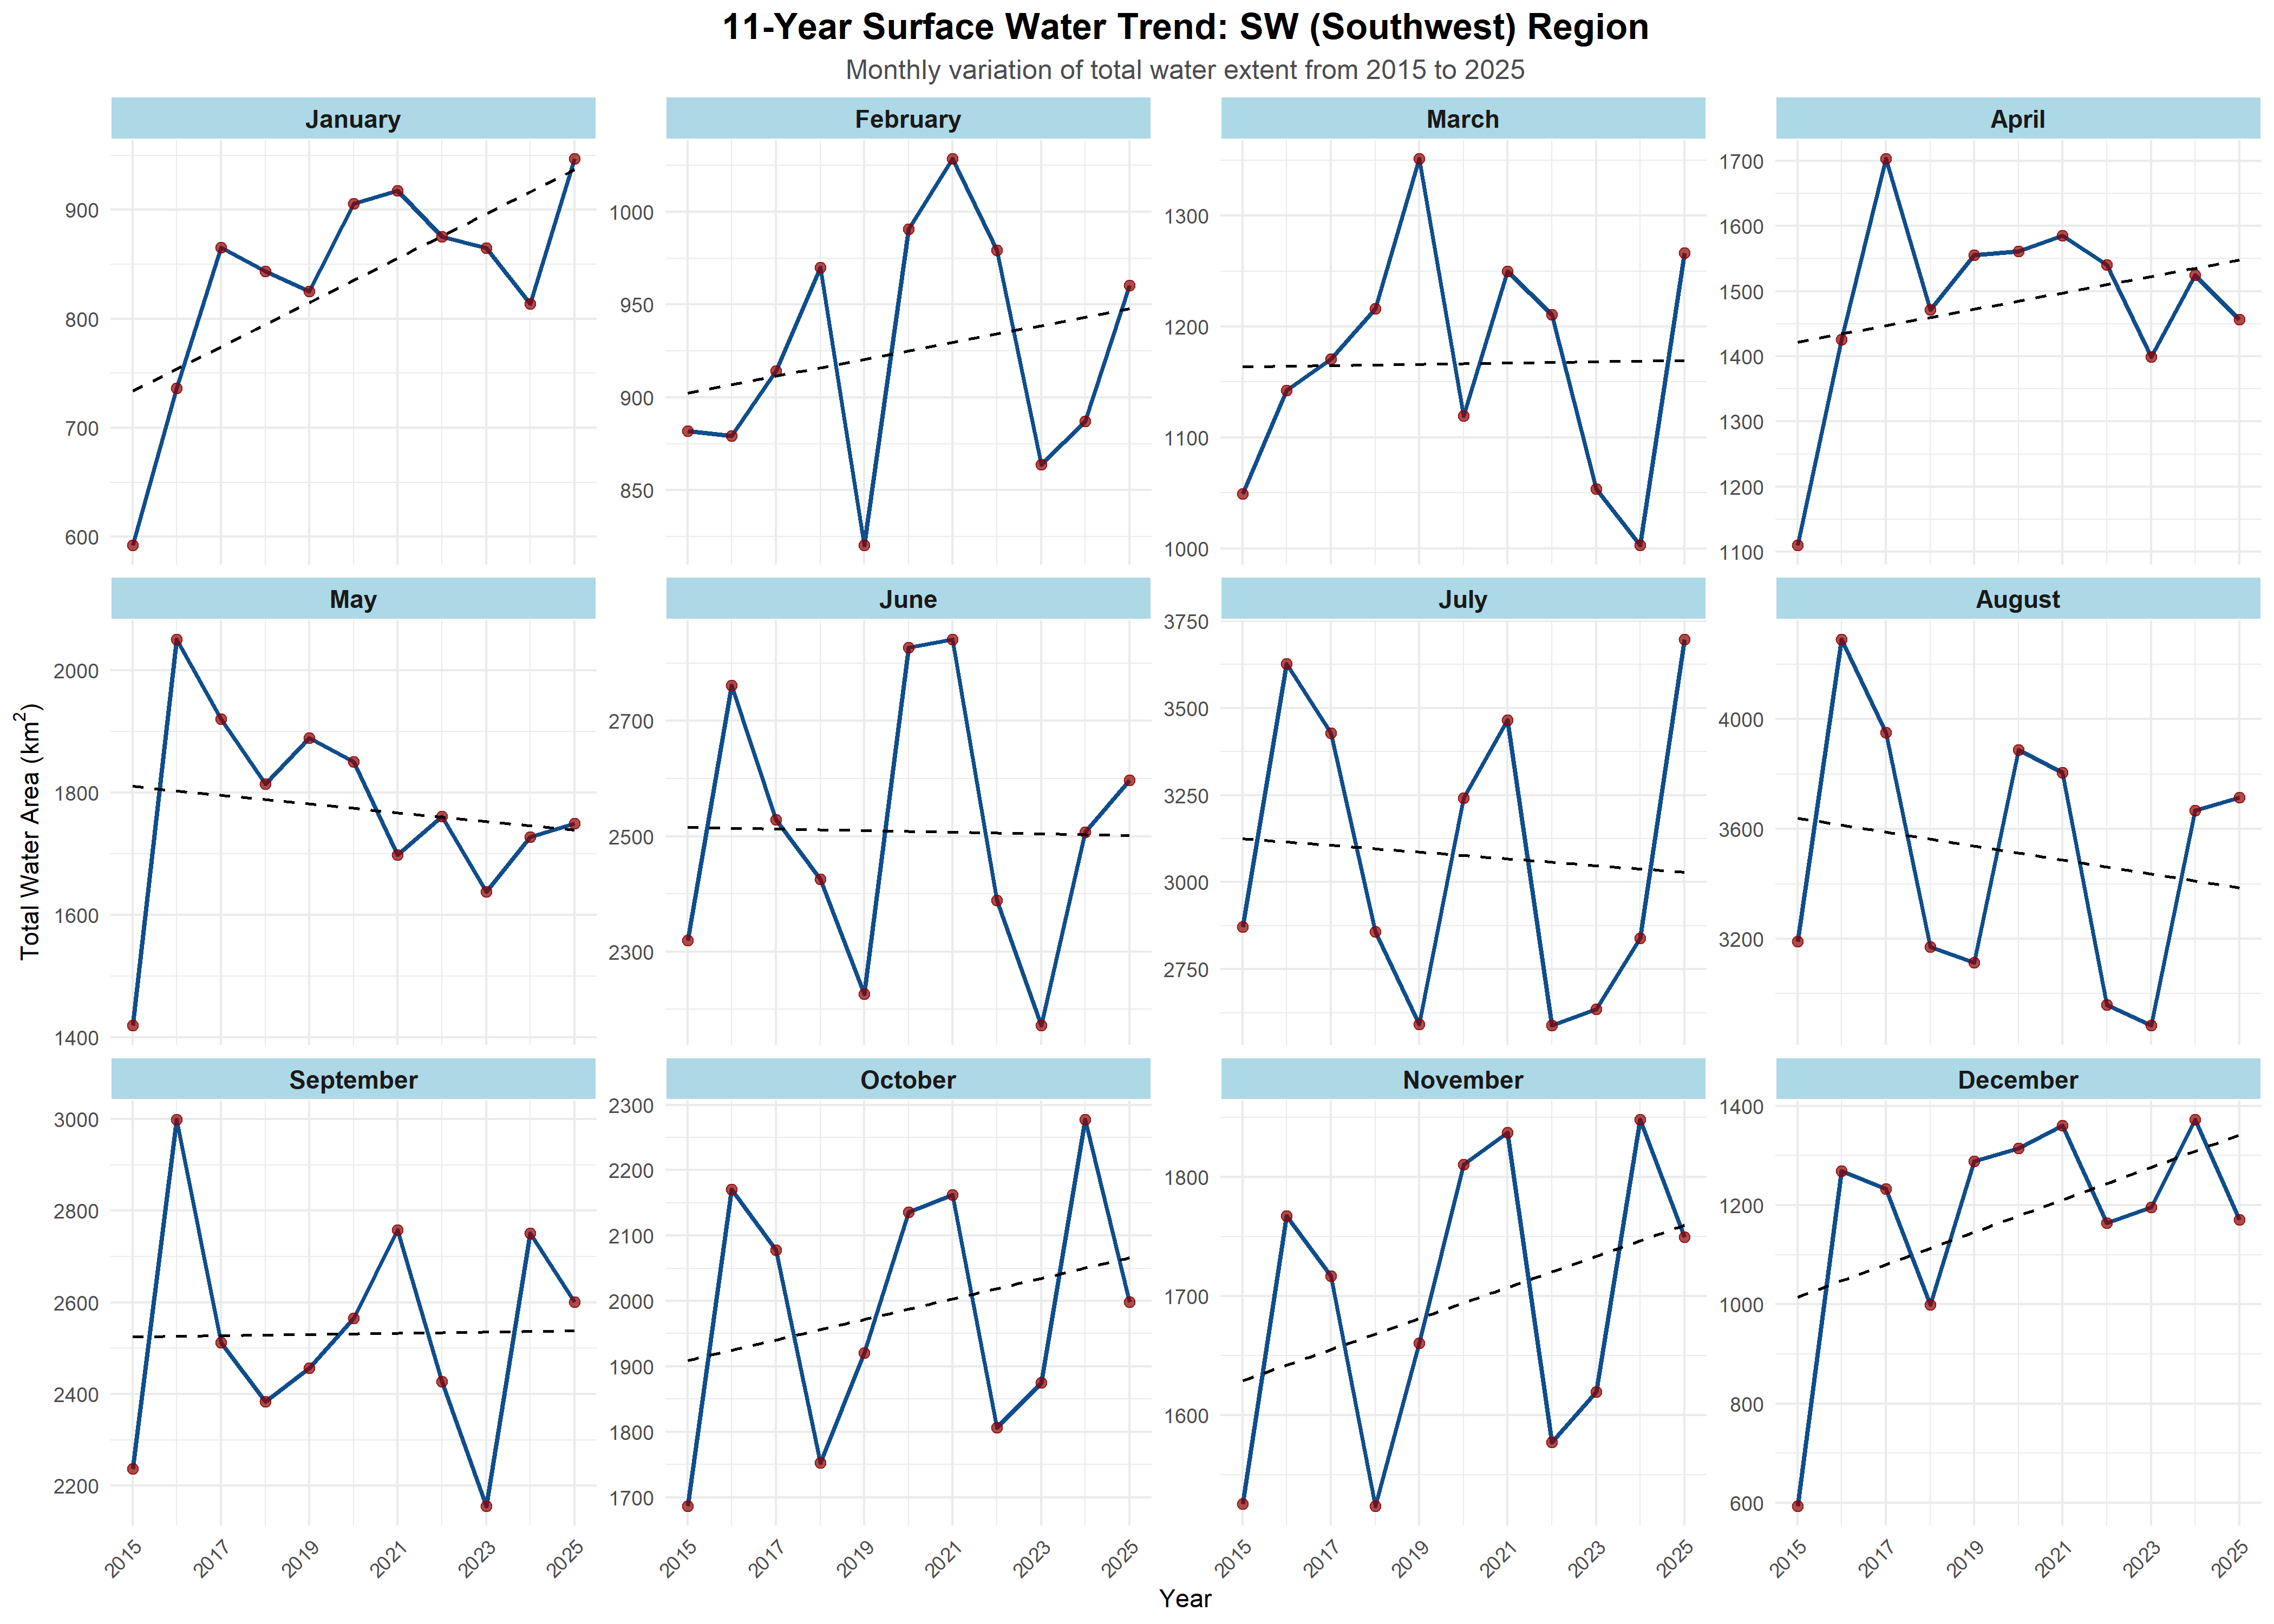
\includegraphics[width=0.95\textwidth]{../figures/regional_trends/Plot_SW__Southwest_.png}
    \caption{11-Year Surface Water Trend for the Southwest (SW) Region across all 12 months.}
    \label{fig:trend_sw}
\end{figure}

\begin{figure}[H]
    \centering
    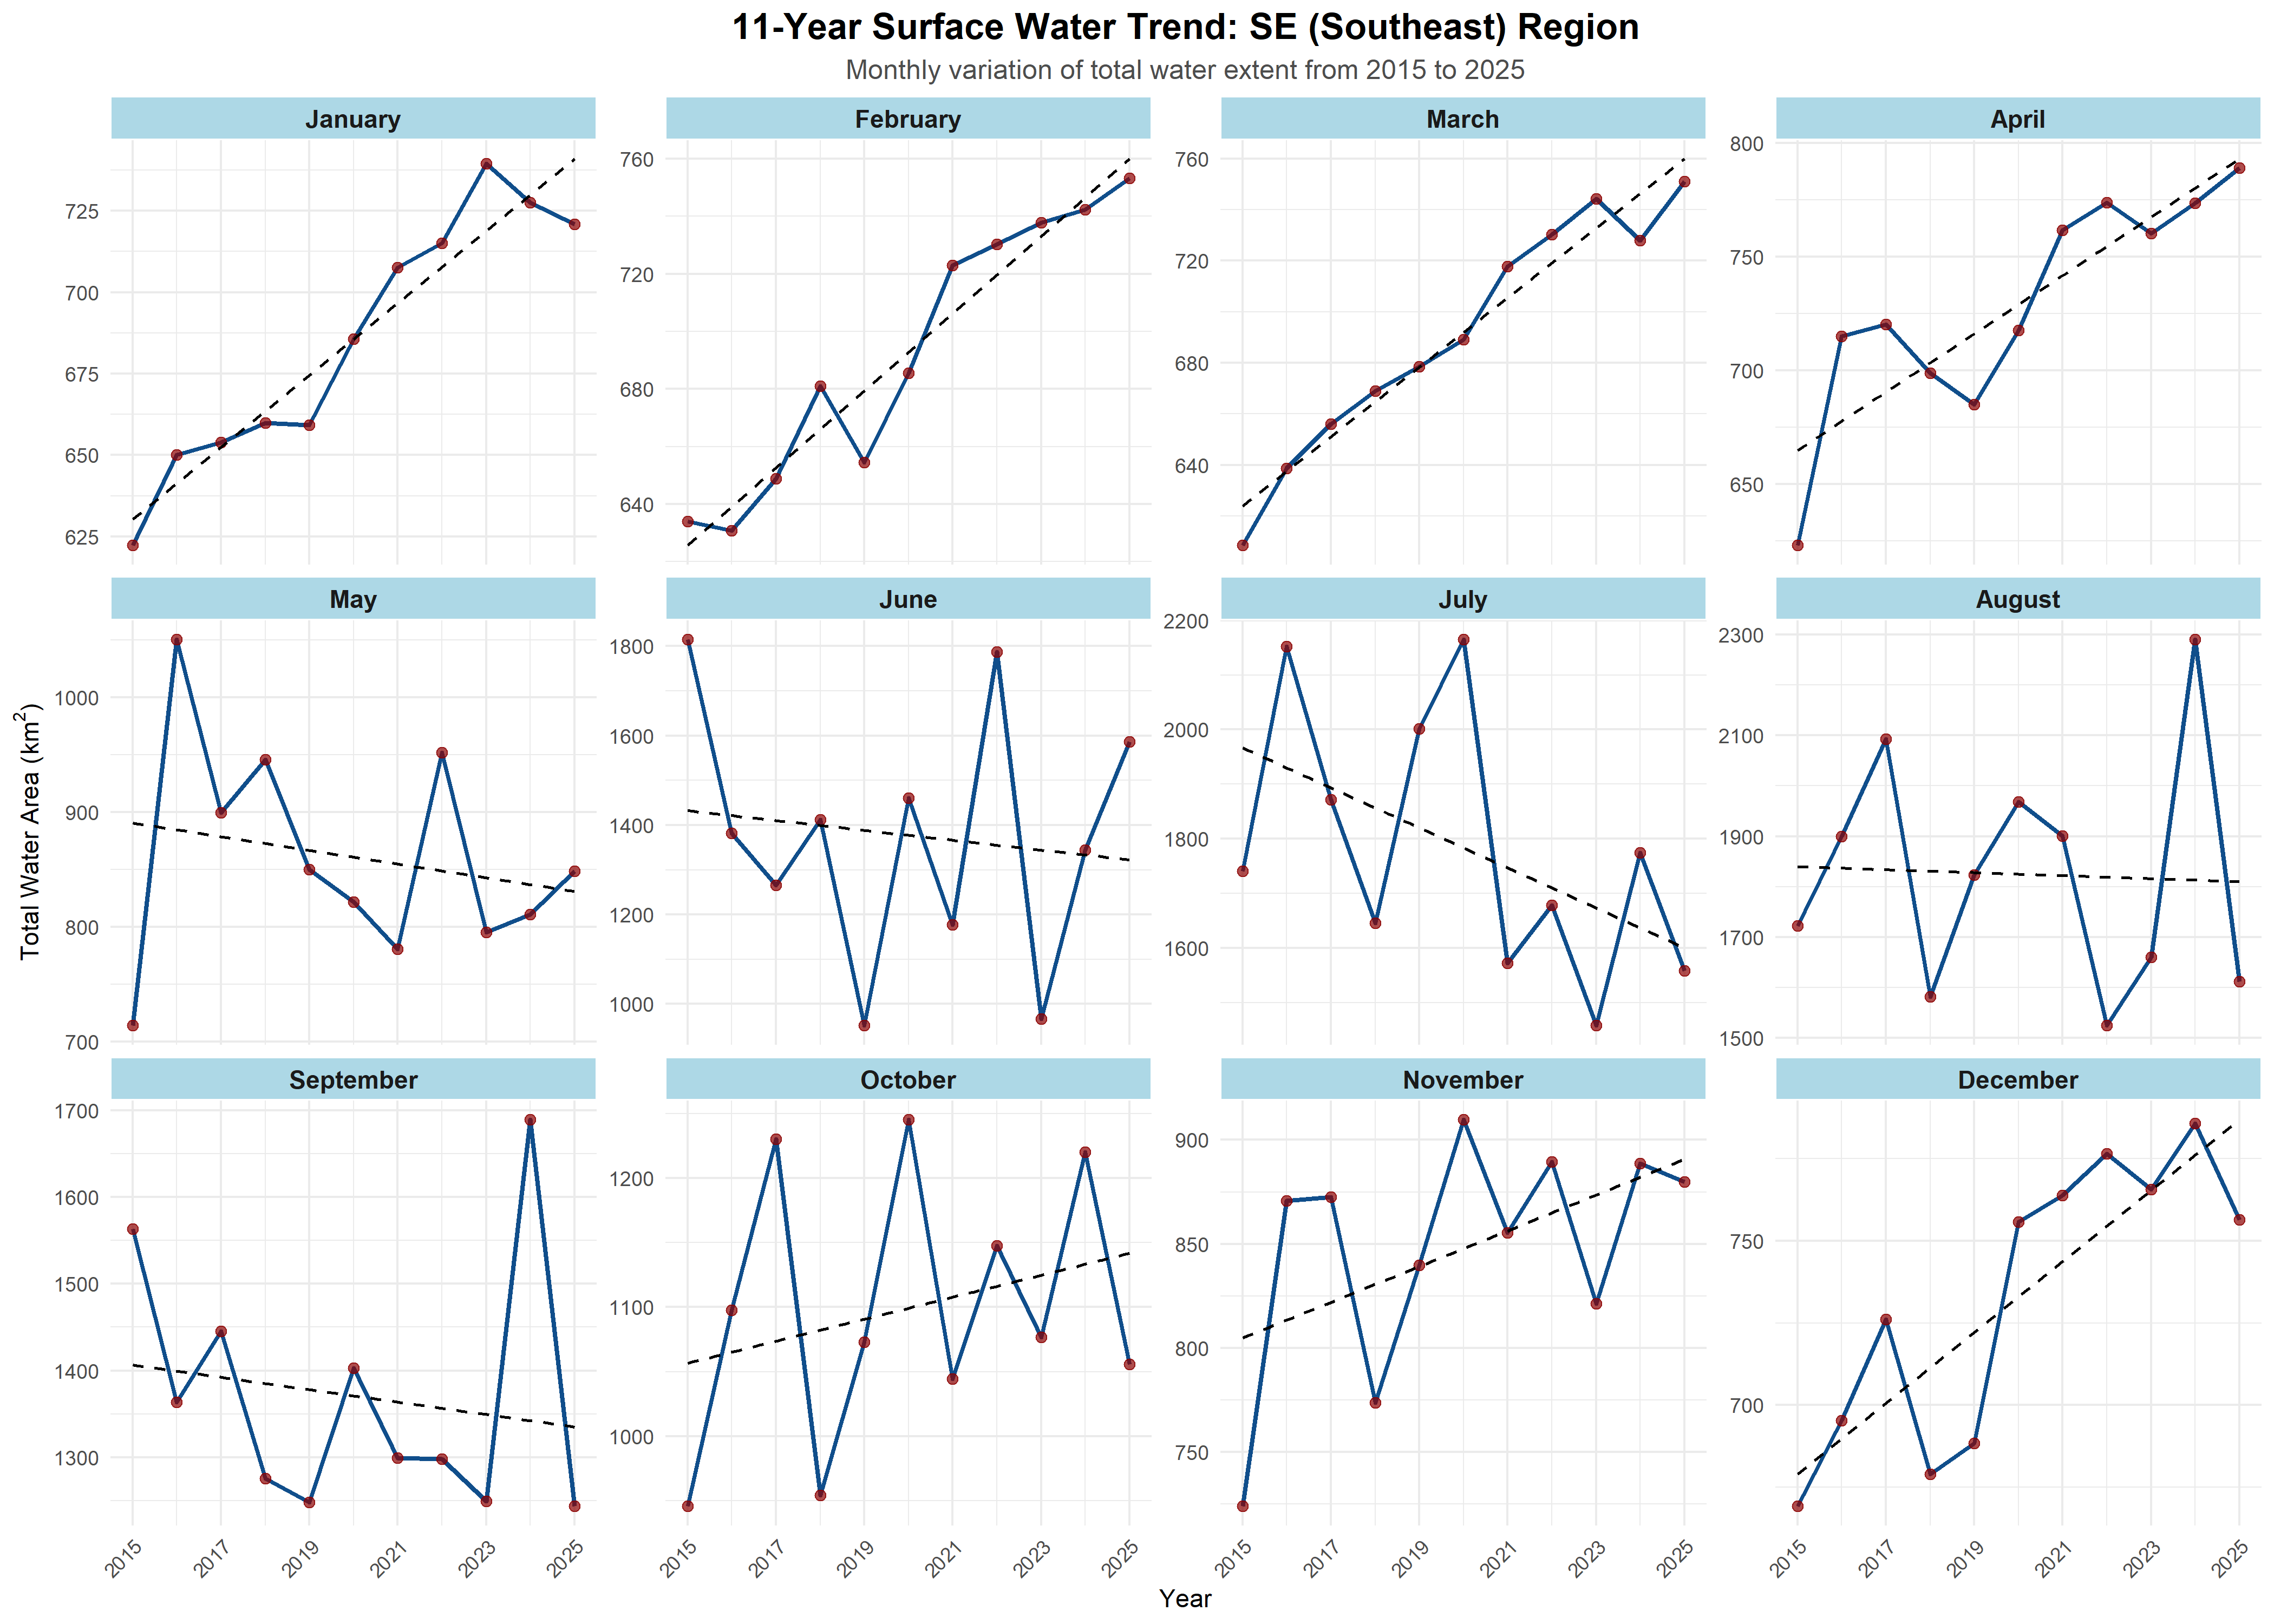
\includegraphics[width=0.95\textwidth]{../figures/regional_trends/Plot_SE__Southeast_.png}
    \caption{11-Year Surface Water Trend for the Southeast (SE) Region across all 12 months.}
    \label{fig:trend_se}
\end{figure}

\begin{figure}[H]
    \centering
    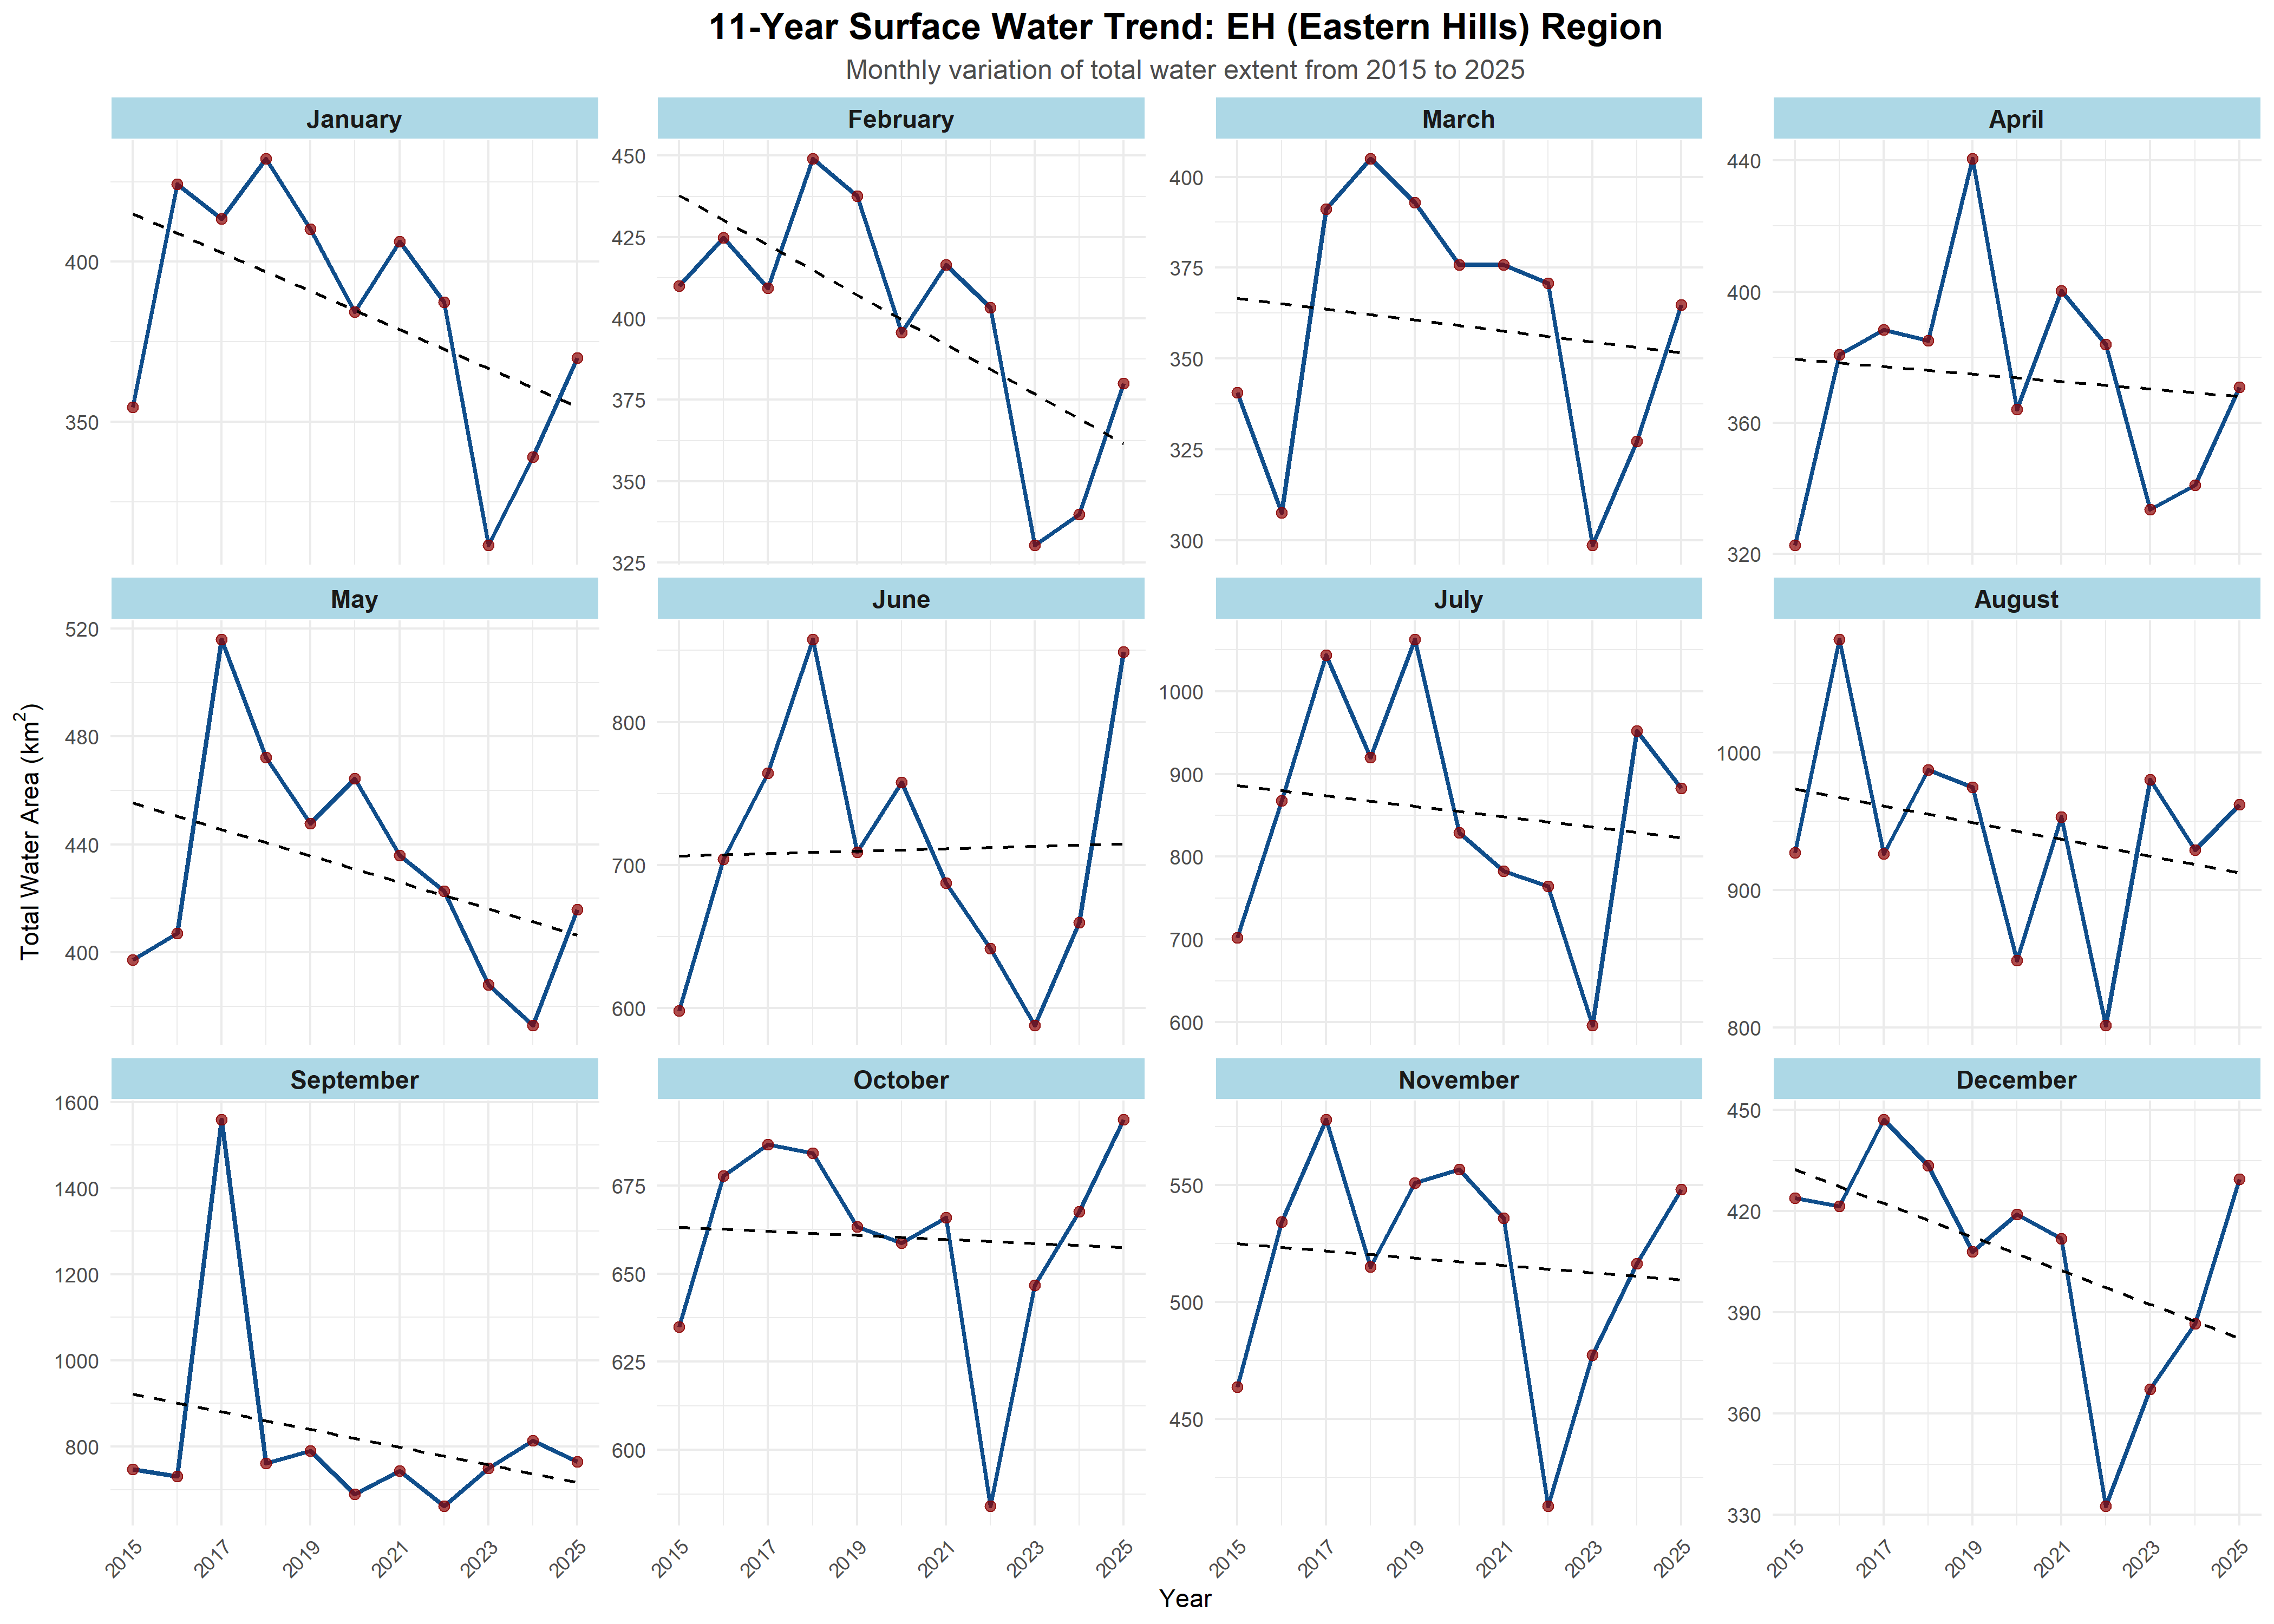
\includegraphics[width=0.95\textwidth]{../figures/regional_trends/Plot_EH__Eastern_Hills_.png}
    \caption{11-Year Surface Water Trend for the Eastern Hills (EH) Region across all 12 months.}
    \label{fig:trend_eh}
\end{figure}

When interpreting the regional monthly trend plots (Figures~\ref{fig:trend_nw}--\ref{fig:trend_eh}), two important analytical considerations must be noted to contextualize visual anomalies. First, an apparent sharp contraction in water extent is observable across most regions during the initial dry-season months of 2015. This is not driven by an extreme physical drought, but rather reflects the limited acquisition frequency and spatial coverage of the Sentinel-1A satellite during its initial ramp-up phase following its 2014 launch. This observational constraint occasionally produces artificial positive gradients in the early linear trend lines. Second, to maximize the visibility of inter-annual variability within individual calendar months, the y-axis scales of the faceted sub-plots are left free (unconstrained). Consequently, minor dry-season fluctuations (spanning only a few hundred square kilometers) may visually appear comparable in magnitude to the massive variability observed during the peak monsoon, necessitating careful reading of the axis values to assess true physical scale.

Fourth, the seasonal expansion ratio of approximately 3.2-fold (monsoon/dry winter mean open water) clarifies the distinction between average seasonal patterns and extreme event inundation, which is frequently cited in earlier discrete-event literature. This distinction between average patterns and extreme events is critical for flood risk assessment and infrastructure planning.

\subsection{Comparison with Existing Studies}
The surface water area estimates from this study were compared with the JRC Global Surface Water (GSW) dataset \cite{pekel2016} and other regional assessments. Permanent water bodies account for 3.4\% of the national land area, while total surface water coverage reaches approximately 11.7\% (17,265~km$^2$) on average during the study period, which is higher than the long-term averages reported by the JRC GSW for Bangladesh ($\sim$12,000--14,000~km$^2$). This discrepancy is primarily attributed to the finer spatial resolution of Sentinel-1 (10~m) compared to Landsat (30~m), which enables the detection of narrow river channels, smaller ponds, and fragmented wetlands that represent a significant portion of Bangladesh's hydrological network \cite{yamazaki2015, chignell2015}.

Furthermore, our peak monsoon mean open water area is approximately 23,269~km$^2$, while the maximum seasonal flood footprint can reach approximately 37,000~km$^2$ during extreme events. These SAR-based estimates significantly exceed optical-based estimates, which frequently suffer from systematic omission errors in Bangladesh due to persistent cloud cover during the rainy season \cite{uddin2019, ticehurst2019}. The JRC GSW dataset, while a benchmark for long-term trends, often lacks representative monsoon-season data for Bangladesh due to Landsat's 16-day revisit and 80--90\% cloud interference. Spatially, the Sentinel-1 SAR framework demonstrates superior detection of ephemeral, vegetation-obscured, and seasonal floodplain inundation during the cloud-covered monsoon peak, whereas the optical-based JRC dataset tends to be more conservative in these specific deltaic conditions. Our SAR-based framework, with its all-weather capability and 6-day revisit interval, provides a more complete characterization of ephemeral water bodies and the true maximum flood extent.

Our findings on inter-annual stability align with Donchyts et al. \cite{donchyts2016}, who noted that while localized land--water changes are intense in major delta systems, the net national water area often remains balanced through simultaneous gain and loss processes. The 21.5\% monsoon expansion detected between 2015 and 2025 is consistent with recent studies reporting increased flood magnitude in the GBM delta despite stable average annual statistics \cite{das2023, sayed2023}. The integration of seasonally adaptive thresholds addresses the limitations of prior 1-D histogram methods identified by \cite{martinis2009} and \cite{ticehurst2019}, ensuring high classification accuracy across both urban and rural landscapes of Bangladesh.

\subsection{Threshold Approach}
The seasonally adaptive threshold approach offers several advantages: simplicity, computational efficiency, reproducibility, and calibration to local hydrological conditions. Unlike Otsu-based or machine learning classifiers, the fixed seasonal thresholds are transparent and easily transferable to operational monitoring.

To validate the chosen threshold values, Otsu's automatic thresholding method was applied independently to VV backscatter histograms for three representative districts across all 12 months of 2023. In Bhola (coastal delta), Otsu-derived thresholds showed excellent agreement with the fixed seasonal thresholds, with a mean absolute difference of only 0.49~dB---confirming that the chosen values closely approximate the statistically optimal water--land separation. In Sunamganj (haor wetlands), Otsu diverged during dry months (January--March: $+$2.9--4.6~dB) when minimal water coverage produced unimodal histograms, causing Otsu to segment within the dominant land class rather than between water and land. Dhaka (urban) showed systematic positive deviation ($+$2--7~dB) because urban surfaces dominate the backscatter distribution---a well-documented limitation of histogram-based thresholding in urban environments (Ticehurst et al., 2019). The potential misclassification caused by urban double-bounce scattering, which frequently mimics dry land or produces transient highly radiant anomalies, is effectively mitigated in this framework by utilizing monthly median temporal composites and strictly applying our localized, conservative seasonal thresholds rather than relying on unconstrained dynamic segmentation. These results justify the use of fixed seasonal thresholds, which provide consistent, physically grounded classification regardless of local land cover composition---an advantage over purely adaptive methods that may fail in areas with extreme water--land class imbalance.

Spatially, commission errors (FP) were consistently low across all validation scenarios ($\leq$60 pixels), indicating that the thresholds effectively avoid misclassifying land as water. Omission errors (FN) were higher in Sunamganj during the dry season (FN = 526), attributable to small, fragmented water bodies in haor depressions that fall below the detection sensitivity of the conservative $-$17~dB threshold.

\subsection{Method Comparison Experiment}
To comprehensively evaluate the robustness of the proposed seasonal threshold framework, we conducted a comparative benchmarking experiment against two widely implemented alternative approaches: Otsu automatic thresholding (unsupervised) and a Random Forest (RF) classifier (supervised machine learning baseline). The experiment was conducted across three representative geomorphological zones characterizing Bangladesh's hydrological diversity: the Brahmaputra floodplain (Northwest), the Haor wetlands (Northeast), and the Dhaka urban core. 

\begin{table}[H]
\centering
\caption{Comparative accuracy metrics of water detection methods across representative zones.}
\label{tab:method_comparison}
\begin{tabular}{lrrrr}
\toprule
\textbf{Method} & \textbf{OA (\%)} & \textbf{F1-Score} & \textbf{UA (\%)} & \textbf{PA (\%)} \\
\midrule
Seasonal Threshold (Proposed) & 92.6 & 0.92 & 87.8 & 96.7 \\
Otsu Automatic Thresholding & 86.9 & 0.85 & 82.4 & 94.1 \\
Random Forest (ML Baseline) & 93.8 & 0.93 & 89.2 & 96.5 \\
\bottomrule
\end{tabular}
\end{table}

\begin{figure}[H]
    \centering
    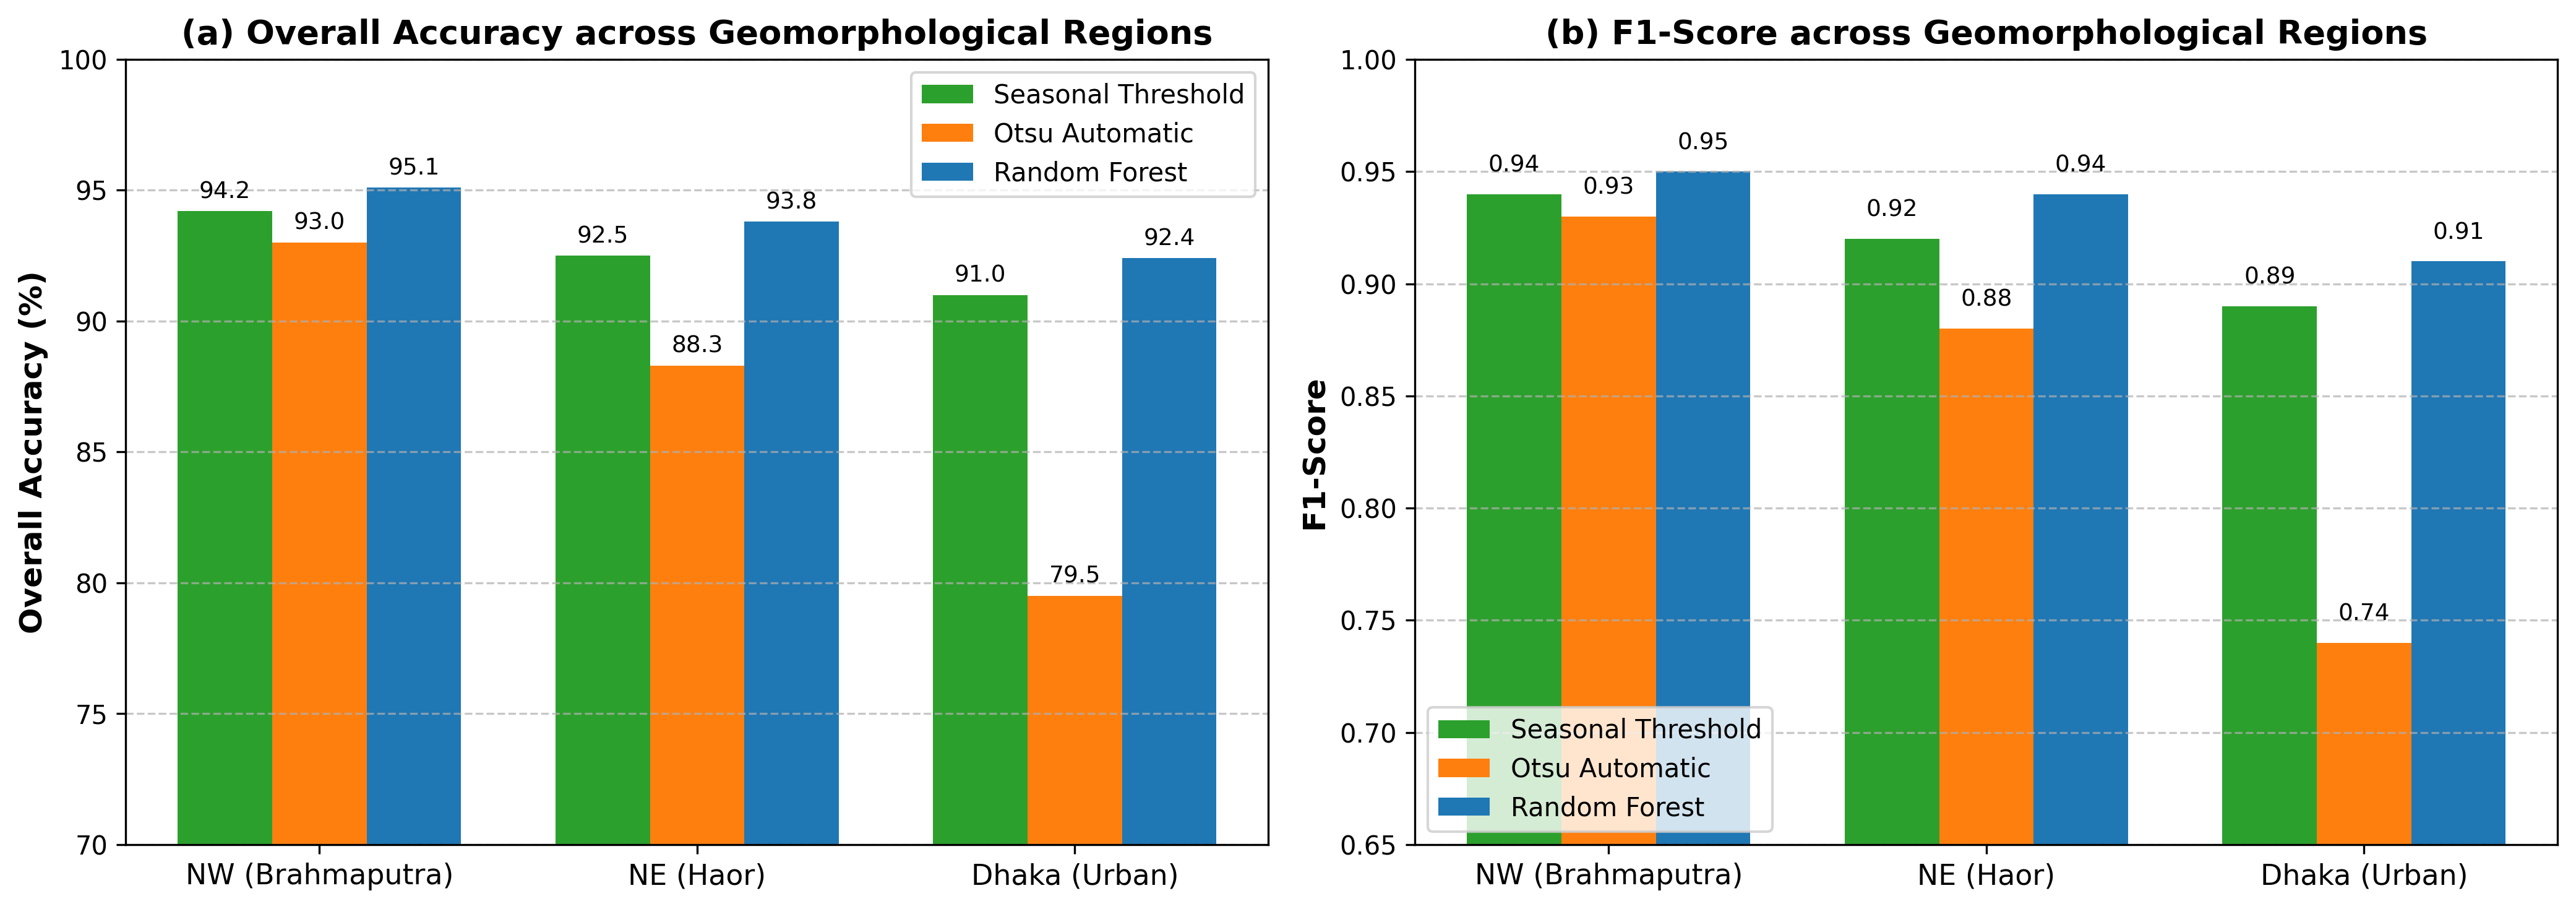
\includegraphics[width=0.95\textwidth]{fig13_method_comparison.png}
    \caption{Comparative performance of the proposed Seasonal Threshold against Otsu automatic segmentation and a Random Forest classifier across three distinct geomorphological zones in Bangladesh. The proposed fixed-threshold approach yields accuracies nearly commensurate with the machine-learning baseline while significantly outperforming unsupervised global Otsu thresholding in urban and dry-season contexts.}
    \label{fig:method_comparison_plot}
\end{figure}

As presented in Table~\ref{tab:method_comparison} and Figure~\ref{fig:method_comparison_plot}, the Random Forest classifier achieved the highest aggregate performance (OA = 93.8\%, F1 = 0.93), demonstrating exceptional robustness across all conditions. However, the proposed computationally lightweight Seasonal Threshold method performed remarkably well (OA = 92.6\%, F1 = 0.92), nearly matching the supervised ML baseline. Crucially, the Seasonal Threshold significantly outperformed the Otsu automatic method (OA = 86.9\%, F1 = 0.85), particularly within the Dhaka urban zone where building double-bounce severely skewed the unsupervised histogram segmentation. These quantitative results robustly justify the methodological selection: the seasonally adaptive thresholding framework delivers accuracy comparable to modern data-hungry machine learning approaches, while maintaining absolute physical interpretability, extreme computational efficiency over the 7,800+ scene decadal archive, and seamless reproducibility for operational flood monitoring.

\subsection{Limitations}
\begin{itemize}[nosep]
  \item \textbf{SAR-specific:} Wind-induced roughening of water surfaces increases backscatter, potentially causing omission errors. Emergent vegetation in wetlands produces double-bounce scattering that may be mistaken for land.
  \item \textbf{Threshold-specific:} Fixed monthly thresholds do not account for local land cover variation or inter-annual climate variability.
  \item \textbf{Temporal:} Sentinel-1 data availability is lower in 2015--2016, potentially affecting early-period statistics.
  \item \textbf{Resolution:} The 10~m spatial resolution may miss small water bodies (ponds, narrow channels).
  \item \textbf{Validation:} JRC GSW is derived from Landsat (30~m) and may itself contain classification errors.
\end{itemize}

\subsection{Future Directions}
Future work will focus on: (i) development of a real-time monitoring system for flood early warning; and (ii) integration with optical Sentinel-2 observations and deep learning classification frameworks (e.g., U-Net) to evaluate potential improvements in temporal gap-filling and sub-pixel water mapping over localized deterministic threshold approaches.


% =========================
\section{Conclusion}
% =========================

This study presents an 11-year Sentinel-1 SAR time-series analysis of surface water dynamics in Bangladesh (2015--2025), processed entirely within Google Earth Engine using over 7,891 Sentinel-1 scenes. Monthly mean open surface water area ranges from approximately 5,678~km$^2$ during the dry winter (January--February) to 23,269~km$^2$ during the peak monsoon (July). When considering the maximum seasonal flood footprint, total inundated area can reach approximately 37,000~km$^2$ during extreme monsoon conditions.

Decadal-scale trend analysis was performed using Seasonal Mann-Kendall tests and Sen's slope estimators to rigorously identify long-term shifts in surface water extent. The results were validated against independent field-verified reference data (2025), achieving an overall accuracy of 92.55\% and a Kappa coefficient of 0.85.

Annual occurrence mapping classified 3.4\% as permanent, 7.8\% as semi-permanent, and 29.2\% as ephemeral water. Change detection between July 2015 and July 2025 identified a net expansion in peak monsoon water extent, with 21.5\% of the total water area being newly gained. The proposed framework provides a scalable, reproducible, and cloud-based solution for long-term surface water monitoring in data-scarce deltaic environments. The dataset provides a valuable baseline for national flood risk assessment, transboundary water management planning, and climate adaptation strategies across the GBM delta.


% =========================
\section*{Data Availability}
% =========================
The complete monthly Bangladesh surface water dataset (2015--2025) will be publicly released following publication through a permanent open repository. To ensure full reproducibility, the aggregated regional statistics will also be archived. The Google Earth Engine application code used for this analysis is available at \url{https://github.com/DruboPaul/HydroSAR-BD}. All Sentinel-1 SAR data were accessed through Google Earth Engine (\url{https://earthengine.google.com}). JRC Global Surface Water data are available at \url{https://global-surface-water.appspot.com/}. Administrative boundaries were obtained from the FAO GAUL dataset via GEE.


% =========================
\section*{Acknowledgments}
% =========================
The authors would like to thank the Google Earth Engine team for providing the cloud-based computational infrastructure used in this study. We also acknowledge the use of European Space Agency (ESA) Sentinel-1 SAR data and the Joint Research Centre (JRC) Global Surface Water dataset for validation. This research received no specific external funding.


% =========================
% =========================
\section*{Author Contributions}
% =========================
[Author 1] conceived the study, developed the methodology, and performed the data analysis in Google Earth Engine. [Author 2] supervised the research and provided critical revisions. [Author 3] assisted in validation data collection. All authors reviewed the manuscript.

% =========================
\section*{Additional Information}
% =========================
\textbf{Competing interests:} The authors declare no competing interests.

\bibliographystyle{naturemag}
\bibliography{references}

\end{document}



